\documentclass[11pt]{amsart}
\usepackage{amsmath,amssymb,amsthm}
\usepackage[margin=1.05in]{geometry}
\usepackage{graphicx}
\usepackage{tikz}
\usetikzlibrary{arrows.meta,positioning,calc}
\graphicspath{{../figures/}}

\numberwithin{equation}{section}
\newtheorem{theorem}{Theorem}[section]
\newtheorem{proposition}[theorem]{Proposition}
\newtheorem{lemma}[theorem]{Lemma}
\newtheorem{corollary}[theorem]{Corollary}
\theoremstyle{definition}
\newtheorem{definition}[theorem]{Definition}
\newtheorem{hypothesis}[theorem]{Hypothesis}
\theoremstyle{remark}
\newtheorem{remark}[theorem]{Remark}
\newtheorem{example}[theorem]{Example}

\newcommand{\Z}{\mathbb{Z}}
\newcommand{\Q}{\mathbb{Q}}
\newcommand{\C}{\mathbb{C}}
\newcommand{\R}{\mathbb{R}}
\newcommand{\N}{\mathbb{N}}
\newcommand{\T}{\mathbb{T}}
\newcommand{\A}{\mathbb{A}}
\newcommand{\hZ}{\widehat{\Z}}
\newcommand{\Prob}{\operatorname{Prob}}
\newcommand{\Gal}{\operatorname{Gal}}
\newcommand{\Cl}{\operatorname{Cl}}
\newcommand{\Frob}{\operatorname{Frob}}
\newcommand{\Ns}{\mathrm{N}}
\newcommand{\OK}{\mathcal{O}_K}
\newcommand{\cA}{\mathcal{A}}
\newcommand{\cO}{\mathcal{O}}
\newcommand{\cF}{\mathcal{F}}
\newcommand{\cG}{\mathcal{G}}
\newcommand{\Idl}{\mathbb{I}}
\newcommand{\pp}{\mathfrak{p}}
\newcommand{\qq}{\mathfrak{q}}
\newcommand{\aaa}{\mathfrak{a}}
\newcommand{\bb}{\mathfrak{b}}
\newcommand{\dd}{\mathfrak{d}}
\newcommand{\mm}{\mathfrak{m}}
\newcommand{\spn}{\operatorname{span}}
\newcommand{\supp}{\operatorname{supp}}
\newcommand{\SG}{\mathcal{SG}}
\newcommand{\Leg}[2]{\left(\frac{#1}{#2}\right)}
\newcommand{\hOS}{\widehat{\cO}_S}

\PassOptionsToPackage{hyphens}{url}
\usepackage[hidelinks,bookmarks=false]{hyperref}
\hypersetup{pdftitle={KMS state uniqueness and phase transitions in localized Bost-Connes systems: from Chebotarev density to the Hardy-Littlewood conjecture},pdfauthor={Ruqing Chen},pdfsubject={Operator algebras; number theory},pdfkeywords={Bost-Connes system, KMS states, phase transitions, Chebotarev density, class field theory}}

\title[KMS uniqueness in localized Bost--Connes systems]{KMS state uniqueness and phase transitions in localized Bost--Connes systems:\\ from Chebotarev density to the Hardy--Littlewood conjecture}
\author{Ruqing Chen}
\address{GUT Geoservice Inc., Montreal, Canada}
\email{ruqing@hotmail.com}
\thanks{DOI: \href{https://doi.org/10.5281/zenodo.22152101}{10.5281/zenodo.22152101}.
Sources, code and data:\newline\url{https://github.com/Ruqing1963/localized-bost-connes}
(this paper: \texttt{paper/}).}
\date{}

\begin{document}

\begin{abstract}
For a number field $K$ and an arbitrary set $S$ of finite primes of $K$ we
study the $S$-local Bost--Connes system $\cA_{K,S}$, whose partition function
is the partial Dedekind product $\zeta_{K,S}(\beta)=\prod_{\pp\in S}(1-\Ns\pp^{-\beta})^{-1}$
and whose symmetry group is $G_S=\Idl_S/\overline{K^\times_{S,+}}$, an
extension of the subgroup $\Cl^+_S$ of the narrow class group generated by $S$
by $U_S/\overline{\cO^\times_{K,+}}$; for $S$ the set of all primes,
$G_S\cong\Gal(K^{ab}/K)$. We classify the $\mathrm{KMS}_\beta$ states
completely and unconditionally, for every $K$, every $S$ and every $\beta>0$:
the simplex is affinely isomorphic to $\Prob(G_S/\Xi_\beta^\perp)$, where
\[
\Xi_\beta(K,S)=\Bigl\{\chi\in\widehat{G_S}:\ \sum_{\pp\in S}\Ns\pp^{-\beta}\bigl(1-\operatorname{Re}\chi(\Frob_\pp)\bigr)<\infty\Bigr\}.
\]
Uniqueness therefore holds if and only if, for every nontrivial finite abelian
extension $L/K$ unramified outside $S\cup\infty$, the primes of $S$ that do not
split completely in $L$ have divergent $\beta$-weighted sum; for $S$ the set of
all primes this is the Chebotarev density theorem, and at $\beta=1$ it is the
non-vanishing $L(1,\chi)\neq0$. The criterion refutes the natural
expectation that uniqueness should follow from the divergence
$\zeta_{K,S}(\beta)=\infty$: we exhibit sets $S$ with
$\zeta_{K,S}(\beta)=\infty$ and with $\sigma(I_S)$ dense in $G_S$ for which the
$\mathrm{KMS}_\beta$ simplex is a segment at every $\beta>0$, the two extreme
points being separated by an explicit pointwise invariant whose almost-everywhere
definedness is a Borel--Cantelli condition. Two mechanisms are isolated: over a
field with $h^+_K>1$ the Hilbert class field supplies obstructing characters
that are everywhere unramified, a phenomenon impossible over $\Q$; and over
$\Q$ the separation between topological density and measure-theoretic
ergodicity is governed by a Kakutani dichotomy. We show that $\beta\mapsto\Xi_\beta$
is non-decreasing and construct systems with any prescribed finite number of
phase transitions. Finally we treat sparse sets: for Brun-summable $S$ with
critical exponent $1$ the partition function is finite at the critical point,
so the low-temperature phase is closed---the opposite of the classical
Bost--Connes system---and for $S=\{2\}\cup\SG$, $\SG$ the Sophie Germain
primes, the existence and location of the transition are equivalent to a
Hardy--Littlewood type density statement.
\end{abstract}

\maketitle
\tableofcontents

\section{Introduction}

The Bost--Connes system \cite{BC} is a $C^*$-dynamical system
$(\cA_{BC},\sigma)$ with partition function $\zeta(\beta)$ and symmetry group
$\hZ^\times\cong\Gal(\Q^{ab}/\Q)$, exhibiting a phase transition at $\beta=1$:
for $0<\beta\le1$ the $\mathrm{KMS}_\beta$ state is unique and of type
$\mathrm{III}_1$; for $\beta>1$ the extremal $\mathrm{KMS}_\beta$ states are of
type $\mathrm I_\infty$ and are permuted freely and transitively by
$\hZ^\times$. Number field analogues were constructed by Ha--Paugam \cite{HP}
and analysed by Laca--Larsen--Neshveyev \cite{LLN}, with $\zeta_K$ in place of
$\zeta$ and $\Gal(K^{ab}/K)$ in place of $\Gal(\Q^{ab}/\Q)$.

This paper studies the systems obtained by replacing the set of all primes by
an arbitrary subset $S$. Two questions organize the analysis. First, when is
the $\mathrm{KMS}_\beta$ state unique? Second, what does the answer depend on?

The received expectation is that uniqueness should be the shadow of the
divergence $\zeta_{K,S}(\beta)=\infty$: when the partition function diverges
there are no Gibbs states, every scaling-invariant measure gives the units
measure zero, and one expects the resulting measure to be forced. We show that
this expectation is false. The correct answer is Theorem~\ref{thm:main}: the
$\mathrm{KMS}_\beta$ simplex is $\Prob(G_S/\Xi_\beta^\perp)$ with $\Xi_\beta$
as in \eqref{eq:Xi} below, so that uniqueness is equivalent to the vanishing of
an obstruction group defined by a convergence condition on a Dirichlet series
indexed by $S$. Divergence of $\zeta_{K,S}(\beta)$ is not enough; what is
needed is that, for each nontrivial character, the primes of $S$ detecting it
are themselves $\beta$-abundant. For $S$ the set of all primes this is supplied
by the Chebotarev density theorem, and the classical uniqueness statement is
recovered; for sparse $S$ it can fail, and we exhibit the failure explicitly.

\subsection*{Main results}

Let $K$ be a number field, $S$ a set of finite primes, $G_S$ the $S$-local
symmetry group of Definition~\ref{def:GS}, and $\sigma:I_S\to G_S$ the
canonical homomorphism from the group of fractional ideals supported on $S$
(Lemma~\ref{lem:coords}). Set
\begin{equation}\label{eq:Xi}
\Xi_\beta(K,S)=\Bigl\{\chi\in\widehat{G_S}:\ \sum_{\pp\in S}\Ns\pp^{-\beta}\bigl|1-\chi(\sigma_\pp)\bigr|^2<\infty\Bigr\}.
\end{equation}

Since $|\chi(\sigma_\pp)|=1$, the summand may be written either way:
\begin{equation}\label{eq:twoforms}
\bigl|1-\chi(\sigma_\pp)\bigr|^2=2\bigl(1-\operatorname{Re}\chi(\sigma_\pp)\bigr)
=2\bigl(1-\operatorname{Re}\chi(\Frob_\pp)\bigr),
\end{equation}
the last step because $\chi(\sigma_\pp)=\chi(\Frob_\pp)^{-1}=\overline{\chi(\Frob_\pp)}$
by Lemma~\ref{lem:frob}. The factor $2$ and the inversion do not affect convergence, so
the form used in the abstract and \eqref{eq:Xi} define the same subgroup.

\begin{itemize}
\item \textbf{Classification} (Theorem~\ref{thm:main}). For every $K$, $S$ and
$\beta>0$, the $\mathrm{KMS}_\beta$ simplex of $\cA_{K,S}$ is affinely
isomorphic to $\Prob\bigl(G_S/\Xi_\beta(K,S)^\perp\bigr)$. Uniqueness holds iff
$\Xi_\beta=\{1\}$; if $\zeta_{K,S}(\beta)<\infty$ then $\Xi_\beta=\widehat{G_S}$
and one recovers the Gibbs states of type $\mathrm I_\infty$ permuted freely
and transitively by $G_S$. The two classical regimes are the two ends of a
single formula.
\item \textbf{Chebotarev criterion} (Theorem~\ref{thm:cheb},
Corollary~\ref{cor:full}). Uniqueness at $\beta$ is equivalent to
\eqref{eq:cheb}: for every nontrivial finite abelian $L/K$ unramified outside
$S\cup\infty$, the primes of $S$ not splitting completely in $L$ have divergent
$\beta$-weighted sum. For $S=P_K$ and $\beta\le1$ this follows from Chebotarev,
and at $\beta=1$ it is exactly $L(1,\chi)\neq0$ (Remark~\ref{rem:Lfunction}).
\item \textbf{Unramified class-group obstruction} (\S\ref{sec:classgp}). If
$h^+_K>1$, characters pulled back from the narrow class group are unramified
everywhere and obstruct uniqueness whenever the primes of $S$ concentrate
$\beta$-negligibly in a proper subgroup. Over $\Q$ this cannot happen: every
obstruction requires a modulus supported on $S$, hence ramification. An
explicit example over $\Q(\sqrt{-5})$ is Example~\ref{ex:sqrt5}.
\item \textbf{Topology versus measure} (\S\ref{sec:density}). Density of
$\sigma(I_S)$ in $G_S$ is necessary but not sufficient for uniqueness. Over
$\Q$ we construct $S=\{3\}\cup P_1\cup R$ with $\sigma(I_S)$ dense, compute
$\Xi_\beta=\{1,\chi\}$ exactly, and exhibit the pointwise invariant
$\Psi$ of \eqref{eq:Psi}; its almost-everywhere definedness is a
Borel--Cantelli condition, while density needs only $R\neq\emptyset$. The
underlying dichotomy is Kakutani's (Remark~\ref{rem:kakutani}). We also show
$\beta\mapsto\Xi_\beta$ is non-decreasing and construct cascades of transitions
(Proposition~\ref{prop:cascade}).
\item \textbf{Sparse sets} (\S\ref{sec:sparse}). The critical inverse
temperature is the convergence exponent $\beta_c(S)$. If
$\sum_{\pp\in S}\Ns\pp^{-\beta_c}<\infty$---which holds for Brun-summable $S$
with $\beta_c=1$---then the type $\mathrm I_\infty$ phase is the \emph{closed}
half-line $[\beta_c,\infty)$ and the partition function does not diverge at the
transition, in contrast with Bost--Connes, where $\beta_c=1$ lies in the type
$\mathrm{III}$ phase (Remark~\ref{rem:sharp}). For $S_\infty=\{2\}\cup\SG$ the
Brun--Halberstam--Richert bound gives $\beta_c\le1$ unconditionally, a lower
bound of Hardy--Littlewood strength gives $\beta_c=1$, and the existence of a
transition is equivalent to $\SG$ having positive convergence exponent
(Theorem~\ref{thm:sg}). We stress in Remark~\ref{rem:noroute} that this is an
encoding, not a method.
\end{itemize}

\subsection*{Conventions}

The Artin map is normalized \emph{arithmetically}: for a finite abelian $L/K$
and a prime $\pp$ unramified in $L$, a uniformizer at $\pp$ (as an idele
trivial elsewhere) is sent to the arithmetic Frobenius $\Frob_\pp$, the
element of $\Gal(L/K)$ inducing $x\mapsto x^{\Ns\pp}$ on the residue field.
All Galois groups are of abelian extensions inside a fixed $K^{ab}$, so
$\Frob_\pp$ is well defined. Sets of primes are always sets of finite primes.
$\Ns$ is the absolute norm. Characters of compact abelian groups are
continuous. The group $G_S$ is compact (Proposition~\ref{prop:GSstructure}) and totally
disconnected---$\Idl_S$ is a totally disconnected locally compact group, so by van Dantzig's
theorem it has a basis of compact open subgroups at the identity, whose images form such a
basis in the Hausdorff quotient $G_S$---hence profinite; so every character of $G_S$ has
finite order (Lemma~\ref{lem:frob}).

Notation for primes is fixed as follows and used without further comment. In the general
number-field setting, primes of $K$ are written $\pp,\qq\in S\subseteq P_K$ with absolute
norm $\Ns\pp$. When a statement is specialized to $K=\Q$---that is, throughout
\S\ref{sec:density} and \S\ref{sec:sparse}---rational primes are written $\ell$ and
$\Ns\ell=\ell$, except that a Sophie Germain prime is written $p$, so that the associated
safe prime is $2p+1$. A fraktur $\pp$ appearing inside a specialized section is always a
back-reference to the general statement being invoked.

Throughout, $S$ is countable, so all the measure spaces below are standard
Borel and disintegrations exist.

\section{The $S$-local system over a number field}\label{sec:system}

\subsection{The symmetry group}

Let $K$ be a number field of degree $d$ over $\Q$, $\OK$ its ring of integers,
$P_K$ the set of nonzero prime ideals. Fix $\emptyset\neq S\subseteq P_K$ and
write:
\begin{itemize}
\item $\hOS=\prod_{\pp\in S}\cO_\pp$, $U_S=\prod_{\pp\in S}\cO_\pp^\times$
(compact);
\item $I_S$ = the group of fractional ideals supported on $S$, free abelian on
$S$; $J_S\subset I_S$ the monoid of integral ones;
\item $\Idl_S=\prod'_{\pp\in S}K_\pp^\times$ (restricted product with respect
to the $\cO_\pp^\times$), with $\operatorname{div}:\Idl_S\twoheadrightarrow I_S$
and $\ker=U_S$;
\item $K^\times_S=\{\alpha\in K^\times: v_\pp(\alpha)=0\ \forall\pp\notin S\}$,
and $K^\times_{S,+}$ its subgroup of totally positive elements, embedded
diagonally in $\Idl_S$.
\end{itemize}

\begin{definition}\label{def:GS}
The \emph{$S$-local symmetry group} is the compact abelian group
\[
G_S:=\Idl_S\big/\overline{K^\times_{S,+}},
\]
with quotient map $r:\Idl_S\to G_S$.
\end{definition}

\begin{remark}\label{rem:closure}
The closure in Definition~\ref{def:GS} is not cosmetic. The diagonal image of
$K^\times_{S,+}$ in $\Idl_S$ is in general not closed: its intersection with $U_S$ has
closure $\overline{\cO^\times_{K,+}}$, the closure of the totally positive units, which by
Proposition~\ref{prop:units} can be a $\Z_p$-module of positive rank. Quotienting by
$K^\times_{S,+}$ itself would leave a non-Hausdorff quotient, and Proposition~\ref{prop:GSstructure}
would fail. Two cases where the distinction disappears: $K=\Q$, where
$\cO^\times_{\Q,+}=\{1\}$ and $\Idl_S=\hZ_S^\times\times\Q^S_{>0}$ splits, so that
$K^\times_{S,+}$ is already closed; and $K$ imaginary quadratic, where $\cO_K^\times$ is
finite. In both, $G_S$ is computed without any limiting process, which is one reason the
phenomena of \S\ref{sec:units} are invisible over $\Q$.
\end{remark}

The choice of $K^\times_{S,+}$ rather than $K^\times_S$ is not a convention: it
is forced by the requirement that for $S=P_K$ one recovers the symmetry group
of \cite{HP,LLN}.

\begin{lemma}\label{lem:gal}
$\A_{K,f}^\times\big/\overline{K^\times_+}\cong\Gal(K^{ab}/K)$, the isomorphism
being induced by the Artin map. By contrast
$\A_{K,f}^\times/\overline{K^\times}$ is the quotient of
$\Gal(K^{ab}/K)$ by the image of $\{\pm1\}^{r_1}$, a proper quotient whenever $K$ has a
real place; for $K=\Q$ it equals $\hZ^\times/\{\pm1\}$.
\end{lemma}

\begin{proof}
By class field theory $\Gal(K^{ab}/K)=\A_K^\times/\overline{K^\times K_\infty^{\times,\circ}}$,
where $K_\infty^\times=\prod_{v\mid\infty}K_v^\times$ and $K_\infty^{\times,\circ}$
is its identity component. Consider the composite
$j:\A_{K,f}^\times\hookrightarrow\A_K^\times\to\Gal(K^{ab}/K)$.

\emph{$j$ is surjective.} Since $K_\infty^\times/K_\infty^{\times,\circ}\cong\{\pm1\}^{r_1}$,
every class is represented by some $(a_f,\varepsilon)$ with
$\varepsilon\in\{\pm1\}^{r_1}$. By weak approximation choose
$\alpha\in K^\times$ whose sign vector at the real places is $\varepsilon$.
Then $(a_f,\varepsilon)\sim(\alpha^{-1}a_f,\ \alpha_\infty^{-1}\varepsilon)$
and $\alpha_\infty^{-1}\varepsilon$ is totally positive, hence lies in
$K_\infty^{\times,\circ}$; so the class equals that of $(\alpha^{-1}a_f,1)$,
which is in the image of $j$.

\emph{$\ker j=\overline{K^\times_+}$.} If $(a_f,1)\in\overline{K^\times K_\infty^{\times,\circ}}$
then, comparing archimedean components, $a_f$ lies in the closure of the set of
$\alpha\in K^\times$ with $\alpha_\infty\in K_\infty^{\times,\circ}$, i.e.\ with
$\alpha$ totally positive. The converse inclusion is clear.

For the second statement, $\A_{K,f}^\times/\overline{K^\times}$ is the further
quotient of $\A_{K,f}^\times/\overline{K^\times_+}$ by the image of $K^\times$,
which is generated by classes of elements of every sign vector; for $K=\Q$,
$\A_f^\times=\hZ^\times\times\Q_{>0}$ and $\Q^\times=\{\pm1\}\times\Q_{>0}$,
giving $\hZ^\times/\{\pm1\}$.
\end{proof}

\begin{corollary}\label{cor:GSfull}
For $S=P_K$ one has $\Idl_{P_K}=\A_{K,f}^\times$ and
$G_{P_K}\cong\Gal(K^{ab}/K)$. For $K=\Q$ and any $S$,
$\Idl_S=\hZ_S^\times\times\Q^S_{>0}$ uniquely, so $G_S=\hZ_S^\times$.
\end{corollary}

\begin{proposition}\label{prop:GSstructure}
Let $\Cl^+_S\le\Cl^+_K$ be the subgroup of the narrow class group generated by
the classes of the primes of $S$, and $\cO^\times_{K,+}$ the group of totally
positive units. Then $K^\times_{S,+}\cap U_S=\cO^\times_{K,+}$ and there is an
exact sequence of compact abelian groups
\begin{equation}\label{eq:exact}
1\longrightarrow U_S\big/\overline{\cO^\times_{K,+}}\longrightarrow G_S\longrightarrow\Cl^+_S\longrightarrow1 .
\end{equation}
\end{proposition}

\begin{proof}
An element of $K^\times_{S,+}$ lying in $U_S$ has trivial divisor, hence is a
totally positive unit. Applying $\operatorname{div}$ gives the surjection of
$G_S$ onto $I_S/P_{S,+}$, where $P_{S,+}$ is the group of principal fractional
ideals with a totally positive generator supported on $S$; by definition
$I_S/P_{S,+}=\Cl^+_S$, a finite group. The kernel is
$U_S/(U_S\cap\overline{K^\times_{S,+}})$, and since $U_S$ is open in $\Idl_S$ one has
$U_S\cap\overline{K^\times_{S,+}}=\overline{U_S\cap K^\times_{S,+}}=\overline{\cO^\times_{K,+}}$.
Compactness follows since $U_S$ is compact and $\Cl^+_S$ finite.
\end{proof}

\begin{figure}[htbp]
\centering
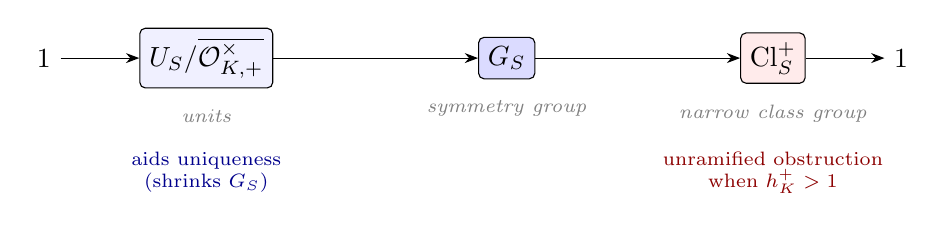
\begin{tikzpicture}[>=Stealth, node distance=6mm]
  \node (one)  {$1$};
  \node[draw, rounded corners=2pt, fill=blue!6, right=10mm of one]  (U)
        {$U_S/\overline{\cO^\times_{K,+}}$};
  \node[draw, rounded corners=2pt, fill=blue!14, right=26mm of U]   (G)
        {$G_S$};
  \node[draw, rounded corners=2pt, fill=red!8,  right=26mm of G]    (C)
        {$\Cl^+_S$};
  \node[right=10mm of C] (two) {$1$};
  \draw[->] (one) -- (U);
  \draw[->] (U)   -- (G);
  \draw[->] (G)   -- (C);
  \draw[->] (C)   -- (two);
  \node[below=1.5mm of U, font=\scriptsize\itshape, gray] (uL) {units};
  \node[below=1.5mm of G, font=\scriptsize\itshape, gray] (gL) {symmetry group};
  \node[below=1.5mm of C, font=\scriptsize\itshape, gray] (cL) {narrow class group};
  \node[below=1.2mm of uL, font=\scriptsize, blue!55!black, align=center]
       {aids uniqueness\\ (shrinks $G_S$)};
  \node[below=1.2mm of cL, font=\scriptsize, red!55!black, align=center]
       {unramified obstruction\\ when $h^+_K>1$};
\end{tikzpicture}
\caption{The two structures in \eqref{eq:exact} that are absent over $\Q$, where both
ends are trivial and $G_S=\hZ_S^\times$. The class group contributes obstructing
characters (\S\ref{sec:classgp}); the units act in the opposite direction
(\S\ref{sec:units}).}
\label{fig:exact}
\end{figure}

\subsection{The algebra and its dynamics}

Ideals of $\OK$ need not be principal, and principal ideals have no canonical
generator; the action of $J_S$ is therefore defined through ideles, with the
ambiguity absorbed by a balanced product.

\begin{definition}\label{def:system}
Let $Y_S=\hOS\times_{U_S}G_S$ be the quotient of $\hOS\times G_S$ by
$(x,g)\sim(wx,\,r(w)^{-1}g)$ for $w\in U_S$; it is a compact metrizable space.
For $\aaa\in J_S$ choose $s\in\Idl_S$ with $\operatorname{div}(s)=\aaa$ and
$s_\pp\in\cO_\pp$ for all $\pp$, and set
\[
\aaa\cdot[x,g]=\bigl[sx,\ r(s)^{-1}g\bigr],
\]
independent of the choice of $s$ because two choices differ by an element of
$U_S$. This is a right action of the abelian monoid $J_S$ by injective
continuous maps with clopen images. The \emph{$S$-local Bost--Connes system} is
the semigroup crossed product
\[
\cA_{K,S}=C(Y_S)\rtimes J_S=\overline{\spn}\bigl\{\mu_\aaa f\mu_\bb^*:\ \aaa,\bb\in J_S,\ f\in C(Y_S)\bigr\},
\]
generated by $C(Y_S)$ and isometries $\mu_\aaa$ with
$\mu_\aaa\mu_\bb=\mu_{\aaa\bb}$, $\mu_\aaa f\mu_\aaa^*=f\circ(\aaa\cdot)^{-1}$
extended by zero, $\mu_\aaa\mu_\aaa^*=\mathbf 1_{\aaa Y_S}$ and
$\mu_\aaa\mu_\bb^*=\mu_\bb^*\mu_\aaa$ for $\aaa,\bb$ coprime. The dynamics is
\[
\sigma_t(f)=f,\qquad\sigma_t(\mu_\aaa)=\Ns\aaa^{\,it}\mu_\aaa .
\]
The group $G_S$ acts by $\theta_h[x,g]=[x,gh^{-1}]$, commuting with $\sigma$.
\end{definition}

For $K=\Q$ this is the system of \cite{LR} restricted to $S$; for $S=P_K$ it is
the system of \cite{HP,LLN}. We record the inductive limit structure, which is
what allows sparse sets to be approached by finite ones.

\begin{proposition}\label{prop:indlim}
If $S=\bigcup_kS_k$ with $S_1\subseteq S_2\subseteq\cdots$, then the maps
$f\mapsto f\circ\mathrm{pr}$, $\mu_\aaa\mapsto\mu_\aaa$ define unital
$\sigma$-equivariant embeddings $\cA_{K,S_k}\hookrightarrow\cA_{K,S_{k+1}}$ and
$\varinjlim_k\cA_{K,S_k}\cong\cA_{K,S}$ equivariantly for
$G_S=\varprojlim_kG_{S_k}$. In particular $\cA_{K,S}\subseteq\cA_{K,P_K}$ for
every $S$.
\end{proposition}

\begin{proof}
The relations are preserved because $\mathbf 1_{\aaa Y_{S'}}$ pulls back to
$\mathbf 1_{\aaa Y_S}$ for $\aaa\in J_S$; injectivity follows from the
gauge-invariant uniqueness theorem, and surjectivity onto a dense subalgebra
from $\hOS=\varprojlim\widehat{\cO}_{S_k}$ together with
$J_S=\bigcup_kJ_{S_k}$ and Stone--Weierstrass. Strong continuity of the limit
dynamics holds on the dense union and hence everywhere.
\end{proof}

\subsection{KMS states are measures}

Let $\varphi$ be a $(\sigma,\beta)$-KMS state. Over $\Q$ one shows
$\varphi(\mu_mf\mu_n^*)=0$ for $m\neq n$ by comparing $m^\beta$ with $n^\beta$;
over a number field this argument is unavailable, because distinct ideals
frequently have equal norms. We use instead the groupoid description.

\begin{proposition}\label{prop:kmsmeasures}
Let $\beta>0$ and set
\[
M_\beta(K,S)=\bigl\{\nu\in\Prob(Y_S):\ \nu(\aaa\cdot E)=\Ns\aaa^{-\beta}\nu(E)\ \ \forall\aaa\in J_S,\ E\ \text{Borel}\bigr\}.
\]
Then $\varphi\mapsto\varphi|_{C(Y_S)}$ is an affine bijection from the
$\mathrm{KMS}_\beta$ simplex of $\cA_{K,S}$ onto $M_\beta(K,S)$. There are no
$\mathrm{KMS}_\beta$ states for $\beta<0$, and for $\beta=0$ the tracial states
correspond to $J_S$-invariant measures.
\end{proposition}

\begin{proof}
$J_S$ is abelian and cancellative, hence an Ore semigroup with enveloping group
$I_S$. By Laca's dilation theorem \cite{Laca} the semigroup crossed product
$\cA_{K,S}=C(Y_S)\rtimes J_S$ is a full corner in the group crossed product
$C_0(\widetilde Y_S)\rtimes I_S$, where
$\widetilde Y_S=\varinjlim(Y_S,\aaa\cdot)$ is the direct limit along the
directed system $J_S$ and $C(Y_S)=\mathbf 1_{Y_S}C_0(\widetilde Y_S)\mathbf 1_{Y_S}$;
the dilation is equivariant for the dynamics, which on the dilation is
implemented by the $\R$-valued cocycle $c(\aaa\bb^{-1})=\log\Ns\aaa-\log\Ns\bb$
on $I_S$. Corner inclusions preserve KMS simplices \cite[\S3]{Laca}, so it
suffices to treat $C_0(\widetilde Y_S)\rtimes I_S=C^*(\cG_S)$, the $C^*$-algebra
of the transformation groupoid $\cG_S=I_S\ltimes\widetilde Y_S$, which is
étale, second countable and locally compact.

By Neshveyev's theorem \cite[Thm.~1.3]{Nesh13}, $\mathrm{KMS}_\beta$ states of
$C^*(\cG_S)$ for the dynamics induced by $c$ are in bijection with pairs
consisting of a probability measure $\nu$ on $\widetilde Y_S^{(0)}$ that is
quasi-invariant with Radon--Nikodym cocycle $e^{-\beta c}$, together with a
$\nu$-measurable field of states on the $C^*$-algebras of the isotropy groups.
Quasi-invariance with that cocycle is exactly
$\nu(\aaa E)=\Ns\aaa^{-\beta}\nu(E)$ for $\aaa\in J_S$.

It remains to see that the isotropy contributes nothing. Taking
$E=\aaa\cdot Y_S$ gives $\nu(\aaa Y_S)=\Ns\aaa^{-\beta}$; applying this to
$\aaa=\pp^k$ and letting $k\to\infty$ gives $\nu(\{x_\pp=0\})=0$ for each
$\pp\in S$, hence, $S$ being countable, $\nu$ is concentrated on the set
$Y_S^\circ$ of classes $[x,g]$ with all $x_\pp\neq0$. On $Y_S^\circ$ the action
of $I_S$ is free: by Lemma~\ref{lem:coords}(2) below, in the coordinates
$(v,g)\in\Z^S\times G_S$ an element $\aaa\bb^{-1}$ acts by
$v\mapsto v+a-b$, and $a=b$ forces $\aaa=\bb$. So $\cG_S$ is principal on a
conull set, all isotropy groups are trivial there, and the field of states is
empty data. The correspondence is affine by construction, and the state is
recovered from $\nu$ by $\varphi=\nu\circ E_S$ with $E_S$ the canonical
conditional expectation onto $C(Y_S)$ given by averaging over the gauge action
of $\widehat{I_S}$.

For $\beta<0$: taking $\aaa\neq(1)$, $\nu(\aaa Y_S)=\Ns\aaa^{-\beta}>1$,
impossible.
\end{proof}

\begin{remark}
Concretely, $\varphi=\nu\circ E_S$ means $\varphi(\mu_\aaa f\mu_\bb^*)=0$ for
$\aaa\neq\bb$ and $\varphi(\mu_\aaa f\mu_\aaa^*)=\nu(f\circ(\aaa\cdot)^{-1})$.
The vanishing for $\aaa\neq\bb$ with $\Ns\aaa=\Ns\bb$, which is invisible to the
modular argument, is here a consequence of freeness of the $I_S$-action, i.e.\
of the fact that ideals, not their norms, index the translations.
\end{remark}

\subsection{Coordinates}

Choose a uniformizer $\pi_\pp$ at each $\pp\in S$. Every $x\in\hOS$ with all
coordinates nonzero factors uniquely as $x_\pp=\pi_\pp^{v_\pp}u_\pp$ with
$v_\pp\in\Z_{\ge0}$, $u_\pp\in\cO_\pp^\times$. Put $V=\Z_{\ge0}^S$. For
$\aaa=\prod\pp^{a_\pp}\in J_S$ let $s_\aaa=(\pi_\pp^{a_\pp})_\pp\in\Idl_S$ and
\begin{equation}\label{eq:sigmadef}
\sigma_\aaa:=r(s_\aaa)^{-1}\in G_S .
\end{equation}

\begin{lemma}\label{lem:coords}
\begin{enumerate}
\item $\aaa\mapsto\sigma_\aaa$ is a monoid homomorphism $J_S\to G_S$ extending
to $\sigma:I_S\to G_S$; its composition with $G_S\to\Cl^+_S$ is the inverse of the natural
surjection $I_S\to\Cl^+_S$, i.e.\ $\sigma_\pp\mapsto[\pp]^{-1}$, the inversion being that of
\eqref{eq:sigmadef}. If $\aaa=(\alpha)$ with $\alpha\in K^\times_{S,+}$ then
$\sigma_\aaa=r(\theta_\alpha)^{-1}$ with $\theta_\alpha:=\alpha^{-1}s_\aaa\in U_S$; for
$K=\Q$, $\sigma_\ell=\theta_\ell$, where $(\theta_\ell)_{\ell'}=\ell$ for $\ell'\neq\ell$
and $1$ for $\ell'=\ell$.
\item $[x,g]\mapsto\bigl(v(x),\,r(u(x))g\bigr)$ is a Borel isomorphism from
$Y_S^\circ$ onto $V\times G_S$, and in these coordinates
$\aaa\cdot(v,g)=(v+a,\ \sigma_\aaa g)$.
\item For every $\nu\in M_\beta(K,S)$ the law $\pi_\beta$ of $v$ is the same:
the $v_\pp$ are independent with $\pi_\beta(v_\pp\ge k)=\Ns\pp^{-k\beta}$, so
$\pi_\beta(v_\pp=k)=(1-\Ns\pp^{-\beta})\Ns\pp^{-k\beta}$.
\item If $(\rho_v)_{v\in V}$ is a disintegration of $\nu$ over $\pi_\beta$,
then $\nu\in M_\beta(K,S)$ if and only if for every $\aaa\in J_S$
\begin{equation}\label{eq:coc}
\rho_{v+a}=(\sigma_\aaa)_*\rho_v\qquad\text{for }\pi_\beta\text{-a.e.\ }v .
\end{equation}
\end{enumerate}
\end{lemma}

\begin{proof}
(1) $s_{\aaa\bb}=s_\aaa s_\bb$, and $r$ is a homomorphism. Composing with
$\operatorname{div}$ modulo $P_{S,+}$ sends $s_\aaa$ to $[\aaa]$, hence $\sigma_\aaa$ to
$[\aaa]^{-1}$. If $\aaa=(\alpha)$ with $\alpha$ totally positive then $\alpha^{-1}s_\aaa$ has
trivial divisor, so lies in $U_S$, and $r(\alpha)=1$ gives
$r(s_\aaa)=r(\alpha^{-1}s_\aaa)$. For $K=\Q$ take $\pi_\ell=\ell$ and $\alpha=\ell$: then
$\theta_\alpha$ has component $\ell^{-1}$ at every $\ell'\neq\ell$ and $1$ at $\ell$, so
$\sigma_\ell=r(\theta_\alpha)^{-1}=\theta_\ell$.

(2) Well-definedness: replacing $(x,g)$ by $(wx,r(w)^{-1}g)$ leaves $v$
unchanged and replaces $u$ by $wu$, so $r(u)g$ is unchanged, $G_S$ being
abelian. The inverse map is $(v,g)\mapsto[(\pi_\pp^{v_\pp})_\pp,g]$. With
$s=s_\aaa$ one has $v\mapsto v+a$, $u\mapsto u$ and
$g\mapsto r(s_\aaa)^{-1}g=\sigma_\aaa g$.

(3) For finite $F\subset S$ and $k_\pp\ge0$, with $\aaa=\prod_{\pp\in F}\pp^{k_\pp}$,
one has $\{v_\pp\ge k_\pp\,\forall\pp\in F\}=\aaa\cdot Y_S$ modulo the null set
$Y_S\setminus Y_S^\circ$, and $\nu(\aaa Y_S)=\Ns\aaa^{-\beta}=\prod_{\pp\in F}\Ns\pp^{-k_\pp\beta}$.
This gives independence and the marginals, hence $\pi_\beta$.

(4) Translation by $a$ multiplies $\pi_\beta$ by the constant $\Ns\aaa^{-\beta}$
by (3). For product sets $A\times B$,
\[
\nu\bigl(\aaa\cdot(A\times B)\bigr)=\int_{A+a}\rho_v(\sigma_\aaa B)\,d\pi_\beta(v),
\qquad
\Ns\aaa^{-\beta}\nu(A\times B)=\int_{A+a}\rho_{v-a}(B)\,d\pi_\beta(v),
\]
the second by the change of variables $v\mapsto v-a$. As $A,B$ are arbitrary,
equality for all of them is \eqref{eq:coc}; the converse is the same
computation with Fubini.
\end{proof}
\section{The classification and the Chebotarev criterion}\label{sec:crit}

Throughout this section $K$, $S$ and $\beta>0$ are fixed, and we work in the
coordinates of Lemma~\ref{lem:coords}. Write $\Ns_\pp:=\Ns\pp$,
$t_\pp:=\Ns\pp^{-\beta}\in(0,1)$, and for $\chi\in\widehat{G_S}$
\[
f_\chi(v):=\widehat{\rho_v}(\chi)=\int_{G_S}\overline{\chi(g)}\,d\rho_v(g),\qquad|f_\chi|\le1 .
\]
By \eqref{eq:coc}, for every $\aaa\in J_S$ with valuation vector $a$,
\begin{equation}\label{eq:fchi}
f_\chi(v+a)=\overline{\chi(\sigma_\aaa)}\,f_\chi(v)\qquad\pi_\beta\text{-a.e.}
\end{equation}
Set $c_\pp:=\overline{\chi(\sigma_\pp)}\in\T$, so that $c^a=\prod_\pp c_\pp^{a_\pp}=\overline{\chi(\sigma_\aaa)}$.

\begin{lemma}[Zero--one law]\label{lem:01}
$|f_\chi|$ is $\pi_\beta$-a.e.\ equal to a constant $c_\chi\in[0,1]$.
\end{lemma}

\begin{proof}
Taking $\aaa=\pp$ in \eqref{eq:fchi} gives $|f_\chi|(v+e_\pp)=|f_\chi|(v)$
a.e. The orbits of $v\mapsto v+e_\pp$ are the fibres of the projection
$V\to\Z_{\ge0}^{S\setminus\{\pp\}}$, so $|f_\chi|$ agrees a.e.\ with a function
not depending on $v_\pp$; that is, $|f_\chi|$ is measurable with respect to
$\sigma(v_{\pp'}:\pp'\neq\pp)$ modulo null sets. Applying this coordinate by
coordinate over a finite set $F$, $|f_\chi|$ is measurable with respect to
$\sigma(v_{\pp'}:\pp'\notin F)$ for every finite $F$, hence with respect to the
tail $\sigma$-algebra of the independent family $(v_\pp)_{\pp\in S}$. By
Kolmogorov's zero--one law that $\sigma$-algebra is $\pi_\beta$-trivial.
\end{proof}

Suppose $\chi\neq1$ and $c_\chi>0$. Then $g:=f_\chi/|f_\chi|$ is a measurable
map $V\to\T$, defined a.e., with
\begin{equation}\label{eq:cob}
g(v+e_\pp)=c_\pp\,g(v)\qquad\pi_\beta\text{-a.e., for every }\pp\in S .
\end{equation}
Put
\[
m_\pp:=\mathbb E_{\pi_\beta}\bigl[c_\pp^{\,v_\pp}\bigr]=\sum_{k\ge0}(1-t_\pp)t_\pp^k c_\pp^k=\frac{1-t_\pp}{1-c_\pp t_\pp}\in\C .
\]

\begin{lemma}\label{lem:mp}
$\displaystyle 1-|m_\pp|^2=\frac{2t_\pp\bigl(1-\operatorname{Re}c_\pp\bigr)}{|1-c_\pp t_\pp|^2}$,
and therefore
\[
\sum_{\pp\in S}\bigl(1-|m_\pp|\bigr)<\infty
\iff
\sum_{\pp\in S}\Ns\pp^{-\beta}\bigl|1-\chi(\sigma_\pp)\bigr|^2<\infty .
\]
\end{lemma}

\begin{proof}
$|m_\pp|^2=(1-t_\pp)^2/|1-c_\pp t_\pp|^2$ and
$|1-c_\pp t_\pp|^2=1-2t_\pp\operatorname{Re}c_\pp+t_\pp^2$ give the identity.
Since $|1-c_\pp|^2=2(1-\operatorname{Re}c_\pp)$ and, for all but at most one
$\pp$ (the one of least norm), $t_\pp$ is bounded away from $1$ by a constant
depending only on $\beta$ and $S$, we get $1-|m_\pp|^2\asymp t_\pp|1-c_\pp|^2$
up to finitely many terms; and $1-|m|\le1-|m|^2\le2(1-|m|)$.
\end{proof}

\begin{proposition}[Necessity]\label{prop:nec}
If $c_\chi>0$ then $\sum_{\pp\in S}(1-|m_\pp|)<\infty$, i.e.\
$\chi\in\Xi_\beta(K,S)$.
\end{proposition}

\begin{proof}
Let $g$ be as in \eqref{eq:cob}, $|g|=1$ a.e. Fix an increasing exhaustion
$F_1\subset F_2\subset\cdots$ of $S$ by finite sets; write
$\cF_F=\sigma(v_\pp:\pp\in F)$ and $P_F=\prod_{\pp\in F}c_\pp^{\,v_\pp}$.

Iterating \eqref{eq:cob} in the coordinate $\pp$ shows that $g\,c_\pp^{-v_\pp}$
agrees a.e.\ with a function not depending on $v_\pp$; doing this for all
$\pp\in F$ shows that $G_F:=g\,P_F^{-1}$ is measurable with respect to
$\sigma(v_\pp:\pp\notin F)$, hence independent of $\cF_F$. Therefore
\[
\mathbb E[g\mid\cF_F]=P_F\,\mathbb E[G_F],\qquad\text{so}\qquad\bigl|\mathbb E[g\mid\cF_F]\bigr|=\bigl|\mathbb E[G_F]\bigr| .
\]
Since $\cF_{F_k}\uparrow\sigma(v)$, martingale convergence gives
$\mathbb E[g\mid\cF_{F_k}]\to g$ in $L^2(\pi_\beta)$, so
$|\mathbb E[G_{F_k}]|\to|g|=1$. For large $k$ put
$\gamma_k=\mathbb E[G_{F_k}]/|\mathbb E[G_{F_k}]|$. Then, as $|P_{F_k}|=1$,
\[
\bigl\|g-\gamma_kP_{F_k}\bigr\|_2^2=\bigl\|G_{F_k}-\gamma_k\bigr\|_2^2=2-2\bigl|\mathbb E[G_{F_k}]\bigr|\longrightarrow0 .
\]
Hence $(\gamma_kP_{F_k})_k$ is Cauchy in $L^2$. For $j<k$, dividing by the
unimodular $P_{F_j}$ and using independence,
\[
\bigl\|\gamma_kP_{F_k}-\gamma_jP_{F_j}\bigr\|_2
=\Bigl\|\gamma_k\!\!\prod_{\pp\in F_k\setminus F_j}\!\!c_\pp^{\,v_\pp}-\gamma_j\Bigr\|_2
\ \ge\ 1-\Bigl|\mathbb E\!\!\prod_{\pp\in F_k\setminus F_j}\!\!c_\pp^{\,v_\pp}\Bigr|
=1-\!\!\prod_{\pp\in F_k\setminus F_j}\!\!|m_\pp| ,
\]
where the inequality is $\|X-\gamma\|_2\ge|\mathbb E X-\gamma|\ge1-|\mathbb E X|$
for unimodular constants $\gamma$. Thus
$\prod_{\pp\in F_k\setminus F_j}|m_\pp|\to1$ as $j,k\to\infty$, the Cauchy
criterion for convergence of $\prod_{\pp\in S}|m_\pp|$ to a nonzero limit, i.e.\
$\sum_\pp(1-|m_\pp|)<\infty$. Lemma~\ref{lem:mp} concludes.
\end{proof}

\begin{proposition}[Sufficiency]\label{prop:suff}
If $\chi\in\Xi_\beta(K,S)$ then there is a measurable $g_\chi:V\to\T$ with
$|g_\chi|=1$ satisfying \eqref{eq:cob}, unique up to a multiplicative constant.
If moreover $\chi\neq1$, there is $\nu\in M_\beta(K,S)$ that is not the
symmetric measure; in particular the $\mathrm{KMS}_\beta$ state is not unique.
\end{proposition}

\begin{proof}
Set $\tilde X_\pp=\overline{(m_\pp/|m_\pp|)}\,c_\pp^{\,v_\pp}$, well defined
because $m_\pp\neq0$; these are independent, unimodular, with
$\mathbb E\tilde X_\pp=|m_\pp|>0$. Put $\tilde P_k=\prod_{\pp\in F_k}\tilde X_\pp$
and $L_k=\prod_{\pp\in F_k}|m_\pp|$; by hypothesis and Lemma~\ref{lem:mp},
$L_k\downarrow L>0$. Then $N_k:=\tilde P_k/L_k$ is an $(\cF_{F_k})$-martingale
with $\|N_k\|_2=1/L_k\le1/L$, hence converges a.s.\ and in $L^2$; so
$\tilde P_k\to g_\chi$ a.s.\ with $|g_\chi|=1$, and passing to the limit in
$\tilde P_k(v+e_\pp)=c_\pp\tilde P_k(v)$ (valid once $\pp\in F_k$) gives
\eqref{eq:cob}. If $g,g'$ both satisfy \eqref{eq:cob} then $g/g'$ is invariant
under all $v\mapsto v+e_\pp$, hence constant by Lemma~\ref{lem:01}.

Now let $\chi\neq1$ and define $\rho_v$ to be the measure on $G_S$ with density
$1+\operatorname{Re}\bigl(g_\chi(v)\chi(g)\bigr)\ge0$ with respect to
normalized Haar measure. It is a probability measure whose Fourier coefficients
$\widehat{\rho_v}(\chi')=\int\overline{\chi'}\,d\rho_v$ are
$\widehat{\rho_v}(1)=1$, $\widehat{\rho_v}(\chi)=\tfrac12g_\chi(v)$,
$\widehat{\rho_v}(\bar\chi)=\tfrac12\overline{g_\chi(v)}$ and $0$ elsewhere when
$\chi^2\neq1$; when $\chi^2=1$ the two coefficients merge into
$\widehat{\rho_v}(\chi)=\operatorname{Re}g_\chi(v)=g_\chi(v)$, which is real because then
all $c_\pp=\pm1$ and all $m_\pp>0$, so that $g_\chi=\lim_k\prod_{\pp\in F_k}c_\pp^{v_\pp}\in\{\pm1\}$.
Since $\widehat{(\sigma_\aaa)_*\rho_v}(\chi')=\overline{\chi'(\sigma_\aaa)}\widehat{\rho_v}(\chi')$,
comparison with $\widehat{\rho_{v+a}}(\chi')$ coefficient by coefficient reduces
to \eqref{eq:cob} for $\chi'=\chi$, to its conjugate for $\chi'=\bar\chi$, and
to $1=1$ or $0=0$ otherwise. So \eqref{eq:coc} holds and
Lemma~\ref{lem:coords}(4) yields $\nu\in M_\beta(K,S)$, with
$\widehat{\rho_v}(\chi)\neq0$, whereas the symmetric measure has $\rho_v$ Haar
and all nontrivial coefficients zero.
\end{proof}

\begin{lemma}\label{lem:subgroup}
$\Xi_\beta(K,S)$ is a subgroup of $\widehat{G_S}$; it equals $\widehat{G_S}$
whenever $\zeta_{K,S}(\beta)<\infty$, and $\beta\mapsto\Xi_\beta$ is
non-decreasing.
\end{lemma}

\begin{proof}
$|1-\chi_1\chi_2(\sigma)|\le|1-\chi_1(\sigma)|+|1-\chi_2(\sigma)|$ and
$(a+b)^2\le2a^2+2b^2$ give closure under products;
$|1-\bar\chi(\sigma)|=|1-\chi(\sigma)|$ under inverses. If
$\sum_\pp\Ns\pp^{-\beta}<\infty$ every $\chi$ qualifies since
$|1-\chi(\sigma_\pp)|\le2$. Monotonicity holds because
$\Ns\pp^{-\beta'}\le\Ns\pp^{-\beta}$ for $\beta\le\beta'$.
\end{proof}

\begin{theorem}[Classification]\label{thm:main}
Let $K$ be a number field, $S$ a nonempty set of finite primes and $\beta>0$.
Then the $\mathrm{KMS}_\beta$ simplex of $\cA_{K,S}$ is affinely isomorphic to
\[
\Prob\bigl(G_S/\Xi_\beta(K,S)^\perp\bigr),\qquad
\Xi_\beta^\perp=\{g\in G_S:\chi(g)=1\ \forall\chi\in\Xi_\beta\}.
\]
In particular:
\begin{enumerate}
\item the $\mathrm{KMS}_\beta$ state is unique if and only if
$\Xi_\beta(K,S)=\{1\}$;
\item if $\zeta_{K,S}(\beta)<\infty$ then $\Xi_\beta=\widehat{G_S}$,
$\Xi_\beta^\perp=\{1\}$, the simplex is $\Prob(G_S)$, its extreme points are the
Gibbs states of the Fock representations, of type $\mathrm I_\infty$, and $G_S$
permutes them freely and transitively;
\item the symmetry $G_S$ acts on the simplex through the quotient
$G_S/\Xi_\beta^\perp$, so $\Xi_\beta^\perp$ is the residual symmetry group of
the phase.
\end{enumerate}
\end{theorem}

\begin{proof}
By Proposition~\ref{prop:kmsmeasures} and Lemma~\ref{lem:coords}, a KMS state
is determined by the family $(\rho_v)$, hence by $(f_\chi)_{\chi\in\widehat{G_S}}$.
By Lemma~\ref{lem:01} and Proposition~\ref{prop:nec}, $f_\chi\equiv0$ for
$\chi\notin\Xi_\beta$. For $\chi\in\Xi_\beta$ let $g_\chi$ be a solution of \eqref{eq:cob} with $|g_\chi|=1$,
unique up to a unimodular constant by Proposition~\ref{prop:suff}. The constants can be
chosen so that $\chi\mapsto g_\chi(v)$ is multiplicative. Indeed, for
$\chi_1,\chi_2\in\Xi_\beta$ the unimodular function $g_{\chi_1}g_{\chi_2}/g_{\chi_1\chi_2}$
satisfies \eqref{eq:cob} with every $c_\pp$ replaced by $1$, hence is invariant under all the
shifts $v\mapsto v+e_\pp$ and is a.e.\ equal to a constant $\omega(\chi_1,\chi_2)\in\T$ by
the argument of Lemma~\ref{lem:01}. The function $\omega$ is a symmetric $2$-cocycle on the
countable abelian group $\Xi_\beta$ with values in the divisible group $\T$; symmetric
cocycles classify abelian extensions, and $\operatorname{Ext}(\Xi_\beta,\T)=0$, so $\omega$
is a coboundary, $\omega(\chi_1,\chi_2)=\lambda(\chi_1)\lambda(\chi_2)/\lambda(\chi_1\chi_2)$
for some $\lambda:\Xi_\beta\to\T$. Replacing $g_\chi$ by $g_\chi/\lambda(\chi)$ gives
$g_{\chi_1}g_{\chi_2}=g_{\chi_1\chi_2}$, whence also $g_1=1$ and
$g_{\bar\chi}=\overline{g_\chi}$. (The explicit normalization
$\lim_k\prod_{\pp\in F_k}\overline{(m_\pp/|m_\pp|)}c_\pp^{v_\pp}$ of
Proposition~\ref{prop:suff} is multiplicative only up to such a cocycle, the arguments of
the $m_\pp$ not being additive in $\chi$.) Then
$f_\chi=\kappa(\chi)g_\chi$ for a scalar $\kappa(\chi)$ with $\kappa(1)=1$, and
$\kappa$ is positive definite on the discrete group $\Xi_\beta$: for
$\chi_i\in\Xi_\beta$, $z_i\in\C$,
\[
\sum_{i,j}z_i\bar z_j\,\kappa(\chi_i\bar\chi_j)
=\mathbb E_{\pi_\beta}\Bigl[\int_{G_S}\Bigl|\sum_iz_i\overline{\chi_i(g)}\,\overline{g_{\chi_i}(v)}\Bigr|^2d\rho_v(g)\Bigr]\ \ge\ 0 .
\]
By Bochner's theorem $\kappa$ is the Fourier transform of a unique probability
measure on the compact dual $\widehat{\Xi_\beta}\cong G_S/\Xi_\beta^\perp$.
Conversely every such measure arises: given $\kappa$ positive definite with
$\kappa(1)=1$, define $\rho_v$ by
$\widehat{\rho_v}(\chi)=\kappa(\chi)g_\chi(v)$ for $\chi\in\Xi_\beta$ and $0$
otherwise; positivity of $\rho_v$ is Bochner again (the function
$\chi\mapsto\kappa(\chi)g_\chi(v)$ is positive definite for each fixed $v$,
being $\kappa$ twisted by the character $\chi\mapsto g_\chi(v)$ of
$\Xi_\beta$), and \eqref{eq:coc} holds by \eqref{eq:cob}. The correspondence
$\nu\leftrightarrow\kappa$ is affine and bijective.

(1) and (3) are immediate. For (2), $\Xi_\beta=\widehat{G_S}$ by
Lemma~\ref{lem:subgroup}, so the simplex is $\Prob(G_S)$; the extreme points
correspond to point masses, and unwinding the correspondence they are the
states $\zeta_{K,S}(\beta)^{-1}\operatorname{Tr}(\pi_g(\cdot)e^{-\beta H})$ in
the Fock representations $\pi_g$ on $\ell^2(J_S)$ determined by $g\in G_S$,
which are irreducible; the action of $G_S$ is translation on the parameter.
\end{proof}

\begin{remark}
Theorem~\ref{thm:main} is a single statement covering both classical regimes.
The high-temperature regime is $\Xi_\beta=\{1\}$ and the low-temperature regime
$\Xi_\beta=\widehat{G_S}$; for the classical systems these are the only two
values that occur, but \S\ref{sec:density} shows that intermediate values do
occur, giving phases with partial symmetry breaking that have no analogue in
\cite{BC,LLN}.
\end{remark}

\subsection{The Chebotarev criterion}

\begin{lemma}\label{lem:frob}
Let $\chi\in\widehat{G_S}$ be nontrivial. Then $\chi$ has finite order and is
trivial on an open subgroup, so there are a finite $F\subset S$ and exponents
$k_\pp\ge1$ with $\chi$ trivial on
$\prod_{\pp\in F}(1+\pp^{k_\pp}\cO_\pp)\times\prod_{\pp\in S\setminus F}\cO_\pp^\times$;
put $\mm=\prod_{\pp\in F}\pp^{k_\pp}$. Let $L/K$ be the finite cyclic extension
attached by class field theory to an extension of $\chi$ to $\Gal(K^{ab}/K)$ trivial on the
inertia groups at all $\pp\notin S$; such extensions exist, and the statements below do not
depend on the choice (see the proof). Then $L$ lies in the ray class field
of conductor dividing $\mm\infty$, hence is unramified outside $S\cup\infty$,
and for every $\pp\in S$ with $\pp\nmid\mm$,
\[
\chi(\sigma_\pp)=\chi(\Frob_\pp)^{-1}.
\]
In particular $\chi(\sigma_\pp)=1$ if and only if $\pp$ splits completely in
$L$.
\end{lemma}

\begin{proof}
First, how $G_S$ sits inside the Galois group. The inclusion $\Idl_S\subset\A_{K,f}^\times$
(ideles with component $1$ outside $S$) composed with the Artin map of Lemma~\ref{lem:gal}
gives a continuous homomorphism $G_S\to\Gal(K^{ab}/K)$, and its composite with the
projection onto $\Gal(K^{S}/K)$, where $K^{S}$ is the maximal abelian extension of $K$
unramified outside $S\cup\infty$, is injective: if $\alpha_nw_n\to s\in\Idl_S$ with
$\alpha_n\in K^\times_+$ and $w_n\in\prod_{\pp\notin S}\cO_\pp^\times$, then, the topology
of $\A_{K,f}^\times$ being that of the restricted product, $\alpha_n$ is eventually a unit at
every $\pp\notin S$, so $\alpha_n\in K^\times_{S,+}$ and $s\in\overline{K^\times_{S,+}}$.
Thus $G_S$ is a closed subgroup of $\Gal(K^{S}/K)$, and $\chi$ extends to a character of
$\Gal(K^{ab}/K)$ trivial on the inertia groups at all $\pp\notin S$. Different extensions
define different fields $L$, but for $\pp\in S$ the element $\Frob_\pp$ is the image of
$s_\pp\in\Idl_S$, so $\chi(\Frob_\pp)$ does not depend on the extension.

$\widehat{G_S}$ is torsion because $G_S$ is a quotient of the totally
disconnected group $\Idl_S$ by a closed subgroup, hence profinite. With the arithmetic
normalization of the Artin map, the idele $s_\pp$ (a uniformizer at $\pp$,
$1$ elsewhere) maps to $\Frob_\pp$ for $\pp$ unramified in $L$; by
\eqref{eq:sigmadef}, $\sigma_\pp=r(s_\pp)^{-1}$, whence the displayed formula.
For $L/K$ abelian, $\Frob_\pp=1$ if and only if $\pp$ splits completely.

Two remarks on the archimedean places. First, $G_S$ is a quotient by the \emph{totally
positive} group $K^\times_{S,+}$, so every character of $G_S$ is trivial on totally
positive elements and the sign conditions at the real places are already absorbed: the
conductor attached to $\chi$ is $\mm\infty$ with the full archimedean part, and $L$ lies
in the \emph{narrow} ray class field of that conductor. This is the same choice that
forces the narrow class group in \eqref{eq:exact}, and it is dictated by
Lemma~\ref{lem:gal}. Second, no archimedean condition enters \eqref{eq:cheb}, which
involves only finite primes; the archimedean part determines which fields $L$ occur, not
the series.
\end{proof}

\begin{theorem}[Chebotarev criterion]\label{thm:cheb}
Let $\beta>0$. The $\mathrm{KMS}_\beta$ state of $\cA_{K,S}$ is unique if and
only if
\begin{equation}\label{eq:cheb}
\sum_{\substack{\pp\in S\\ \pp\ \text{not split completely in }L}}\Ns\pp^{-\beta}=\infty
\end{equation}
for every finite abelian extension $L/K$ inside $K^{ab}$, unramified outside
$S\cup\infty$, whose associated character of $G_S$ is nontrivial.
\end{theorem}

\begin{proof}
By Theorem~\ref{thm:main}(1) uniqueness means $\Xi_\beta=\{1\}$. By
Lemma~\ref{lem:frob}, for nontrivial $\chi$ the quantity
$|1-\chi(\sigma_\pp)|^2$ vanishes exactly on the primes of $S$ splitting
completely in $L$ and is at least $\min_{\omega\neq1}|1-\omega|^2>0$ elsewhere,
$\omega$ ranging over the finitely many values of $\chi$; the finitely many
$\pp\mid\mm$ do not affect convergence. Hence $\chi\notin\Xi_\beta$ is exactly
\eqref{eq:cheb}.
\end{proof}

\begin{corollary}[The classical systems]\label{cor:full}
Let $S=P_K$ and $0<\beta\le1$. Then $\Xi_\beta(K,P_K)=\{1\}$, so the
$\mathrm{KMS}_\beta$ state of the Bost--Connes system of $K$ is unique. For
$\beta>1$, $\zeta_K(\beta)<\infty$ and Theorem~\ref{thm:main}(2) gives the
extremal Gibbs states permuted freely and transitively by $\Gal(K^{ab}/K)$.
\end{corollary}

\begin{proof}
Let $L/K$ be nontrivial abelian of degree $m\ge2$. By the Chebotarev density
theorem the primes of $K$ not splitting completely in $L$ have natural density
$1-1/m\ge\tfrac12$, so $\sum\Ns\pp^{-1}=\infty$ over that set, hence
$\sum\Ns\pp^{-\beta}=\infty$ for $\beta\le1$. Apply Theorem~\ref{thm:cheb}. The
second statement uses $\zeta_K(\beta)<\infty$ for $\beta>1$ and
Corollary~\ref{cor:GSfull}.
\end{proof}

\begin{remark}[$L$-functions]\label{rem:Lfunction}
For a nontrivial ray class character $\chi$ mod $\mm$ and $\beta>1$,
\[
\log\zeta_{K,S}(\beta)-\operatorname{Re}\log L_S(\beta,\chi)
=\sum_{\pp\in S}\Ns\pp^{-\beta}\bigl(1-\operatorname{Re}\chi(\pp)\bigr)+O(1),
\]
the error absorbing higher prime powers. So $\chi\in\Xi_\beta$ says exactly that
$\log|L_S(\beta,\chi)|$ tracks $\log\zeta_{K,S}(\beta)$ to within a bounded
error. For $S=P_K$ and $\beta\downarrow1$ the left side tends to $+\infty$,
because $\zeta_K$ has a simple pole at $\beta=1$ while $L(\beta,\chi)\to L(1,\chi)\neq0$.
Thus the uniqueness half of the Bost--Connes theorem for $K$ is, in this
formulation, precisely the non-vanishing $L(1,\chi)\neq0$ of Hecke \cite{Hecke} and Landau \cite{Landau}
(see also \cite[Ch.~VII]{Neu});
over $\Q$ it is Dirichlet's theorem. Chebotarev enters as the density-theoretic
form of the same input.
\end{remark}

\begin{remark}[Primes of degree $\ge2$ are negligible]\label{rem:degree}
At most $d=[K:\Q]$ primes lie above each rational prime, so
$\sum_{\deg\pp\ge2}\Ns\pp^{-\beta}\le d\sum_pp^{-2\beta}<\infty$ for
$\beta>\tfrac12$. Hence for $\beta>\tfrac12$ the group $\Xi_\beta(K,S)$ is
unchanged if $S$ is replaced by its set of degree-one primes, and all
obstructions in the range of interest are carried by primes with $\Ns\pp=p$.
\end{remark}

\subsection{Failure of the ergodicity hypothesis}

It is natural to hope that whenever $\zeta_{K,S}(\beta)=\infty$---so that the
units carry measure zero and no Gibbs state exists---the action of
$K^\times_{S,+}$ on $\hOS$ is ergodic for every $\nu\in M_\beta(K,S)$, whence
uniqueness. This is how the classical uniqueness theorem is proved in
\cite{Nesh02}. Theorem~\ref{thm:main} shows the hope is unfounded in general.

\begin{example}[Non-uniqueness with divergent partition function]\label{ex:first}
Let $K=\Q$ and $S=\{3\}\cup\{\ell\equiv1\ (\mathrm{mod}\ 3)\}$. Then
$\sum_{\ell\in S}\ell^{-1}=\infty$, so $\zeta_S(\beta)=\infty$ for $\beta\le1$.
Let $\chi$ be the quadratic character of $\Z_3^\times$, regarded as an element
of $\widehat{G_S}=\widehat{\hZ_S^\times}$ supported at the component $3$. For
$\ell\in S$, $\ell\neq3$, one has $(\sigma_\ell)_3=\ell\equiv1\bmod3$, so
$\chi(\sigma_\ell)=1$; and $(\sigma_3)_3=1$, so $\chi(\sigma_3)=1$. Hence the
sum in \eqref{eq:Xi} vanishes identically and $\chi\in\Xi_\beta$ for every
$\beta>0$. By Theorem~\ref{thm:main} the $\mathrm{KMS}_\beta$ state is never
unique, although there are no Gibbs states for $\beta\le1$.

Here $\sigma(I_S)$ is contained in the proper closed subgroup $\ker\chi$, so
the failure is already visible topologically. Section~\ref{sec:density} gives
examples where it is not.
\end{example}

\begin{remark}
The correct general statement replacing the ergodicity hypothesis is
Theorem~\ref{thm:cheb}. What the classical proof uses is not the divergence of
$\zeta_{K,S}$ but the equidistribution of $S$ in ray classes; the two coincide
for $S=P_K$ and diverge for sparse $S$.
\end{remark}
\section{Algebraic obstructions and the separation of topology and measure}\label{sec:obstructions}

Theorem~\ref{thm:cheb} reduces uniqueness to a statement about how the primes
of $S$ are distributed among Frobenius classes. Two independent mechanisms can
make it fail. The first is arithmetic and specific to fields of narrow class
number $>1$; the second is measure-theoretic and occurs already over $\Q$.

\subsection{The unramified class-group obstruction}\label{sec:classgp}

Over $\Q$ every nontrivial character of $G_S=\hZ_S^\times$ is built from the
components at finitely many primes \emph{of $S$}: the modulus must be supported
on $S$, and the associated field is ramified there. Over a field with
$h^+_K>1$ this is no longer so, because \eqref{eq:exact} provides a surjection
$G_S\twoheadrightarrow\Cl^+_S$ whose characters are trivial on all local units.

\begin{proposition}\label{prop:unram}
Let $\psi$ be a character of $\Cl^+_S$ and $\chi=\psi\circ(G_S\to\Cl^+_S)$. Then
$\chi(\sigma_\pp)=\psi([\pp])^{-1}=\overline{\psi([\pp])}$ for every $\pp\in S$, the field $L$ attached to
$\chi$ is contained in the narrow Hilbert class field $H^+$ of $K$ and is
therefore unramified at all finite primes, and
\[
\chi\in\Xi_\beta(K,S)\iff\sum_{\substack{\pp\in S\\ [\pp]\notin\ker\psi}}\Ns\pp^{-\beta}<\infty .
\]
Consequently, if for some proper subgroup $H<\Cl^+_S$ the primes of $S$ lying
outside $H$ form a $\beta$-summable set, then the $\mathrm{KMS}_\beta$ state of
$\cA_{K,S}$ is not unique, and no ramified data is involved.
\end{proposition}

\begin{proof}
Lemma~\ref{lem:coords}(1) identifies the image of $\sigma_\pp$ in $\Cl^+_S$ with
$[\pp]^{-1}$, and inversion does not affect $|1-\chi(\sigma_\pp)|$; the rest is Theorem~\ref{thm:main} together with the
computation in the proof of Theorem~\ref{thm:cheb}. Characters of $\Cl^+_K$
correspond to subfields of $H^+$ by class field theory.
\end{proof}

\begin{example}[$K=\Q(\sqrt{-5})$]\label{ex:sqrt5}
Here $h_K=h^+_K=2$ (there are no real places, so the narrow and wide class
groups agree), $\cO_K^\times=\{\pm1\}$ is finite, and $H=K(i)$. For a rational
prime $p\neq2,5$ split in $K$, the primes above $p$ are principal iff
$p=x^2+5y^2$ iff $p\equiv1,9\pmod{20}$, and non-principal iff $2p=x^2+5y^2$
iff $p\equiv3,7\pmod{20}$.

Let $S_0=\{\pp:\deg\pp=1,\ [\pp]=1\}$ and let $R=\{\pp_1,\pp_2,\dots\}$ be an
infinite set of degree-one primes with $[\pp]\neq1$, chosen so sparsely that
$\Ns\pp_k>2^{2^k}$; put $S=S_0\cup R$. Then:
\begin{enumerate}
\item $\sum_{\pp\in S}\Ns\pp^{-1}=\infty$, since by Chebotarev the rational
primes $\equiv1,9\pmod{20}$ have positive density; hence $\beta_c(K,S)=1$ and
$\zeta_{K,S}(\beta)=\infty$ for $0<\beta\le1$;
\item $\sum_{\pp\in R}\Ns\pp^{-\beta}\le\sum_k2^{-\beta2^k}<\infty$ for every
$\beta>0$;
\item with $\psi$ the nontrivial character of $\Cl_K\cong\Z/2\Z$ and
$\chi=\psi\circ(G_S\to\Cl_S)$---note $\Cl_S=\Cl_K$ because $R\neq\emptyset$---
Proposition~\ref{prop:unram} gives
$\sum_{\pp\in S}\Ns\pp^{-\beta}|1-\chi(\sigma_\pp)|^2=4\sum_{\pp\in R}\Ns\pp^{-\beta}<\infty$,
so $\chi\in\Xi_\beta(K,S)$ for every $\beta>0$;
\item $\sigma(I_S)$ is dense in $G_S$ (Proposition~\ref{prop:densesqrt5}).
\end{enumerate}
Hence for every $\beta\in(0,1]$ the $\mathrm{KMS}_\beta$ simplex of $\cA_{K,S}$
is a segment with exactly two extreme points, neither of them a Gibbs state,
and $G_S$ acts on them through $G_S/\ker\chi\cong\Z/2\Z$. The symmetry is
partially broken at every temperature, and the obstruction is everywhere
unramified.
\end{example}

\begin{proposition}\label{prop:densesqrt5}
With $S$ as in Example~\ref{ex:sqrt5}, $\sigma(I_S)$ is dense in $G_S$.
\end{proposition}

\begin{proof}
$G_S=\varprojlim_\mm G_S/r(W_\mm)$ where
$W_\mm=\prod_{\pp\in F}(1+\pp^{k_\pp}\cO_\pp)\times\prod_{\pp\in S\setminus F}\cO_\pp^\times$
runs over the open subgroups of the above form, so it suffices to prove
surjectivity onto each finite quotient $C_\mm:=G_S/r(W_\mm)$. By
Definition~\ref{def:GS} and \eqref{eq:exact}, $C_\mm$ is a quotient of the ray
class group $\Cl_\mm(K)$ in which the image of $\sigma_\pp$ is the class of
$\pp$ for $\pp\nmid\mm$; so we must show that
$\{[\pp]_{C_\mm}:\pp\in S,\ \pp\nmid\mm\}$ generates $C_\mm$.

Let $C^\circ_\mm=\ker(C_\mm\to\Cl_K)$, of index $1$ or $2$. By the Chebotarev
density theorem applied to the ray class field of conductor $\mm$, every class
of $C^\circ_\mm$ contains infinitely many degree-one primes; each such prime is
principal in $\Cl_K$, hence lies in $S_0\subseteq S$, and all but finitely many
avoid $F$. So the generated subgroup contains $C^\circ_\mm$. If
$C^\circ_\mm=C_\mm$ we are done. Otherwise choose $\pp\in R\setminus F$, which
exists as $R$ is infinite; its class lies outside $C^\circ_\mm$ because
$[\pp]\neq1$ in $\Cl_K$, and the index is $2$, so the generated subgroup is all
of $C_\mm$.
\end{proof}

\subsection{Density is not enough}\label{sec:density}

We now work over $K=\Q$, where $G_S=\hZ_S^\times$ and, by Lemma~\ref{lem:coords}(1),
$\sigma_\ell=\theta_\ell$ with $(\theta_\ell)_{\ell'}=\ell$ for
$\ell'\neq\ell$ and $1$ for $\ell'=\ell$; we write $\Theta_S=\sigma(I_S)$. The
next results show that density of $\Theta_S$ in $G_S$---the topological form of
the ergodicity hypothesis---is necessary but not sufficient.

\begin{lemma}\label{lem:densenec}
If $\overline{\sigma(I_S)}\neq G_S$ then $\Xi_\beta(K,S)\neq\{1\}$ for every
$\beta>0$, and the $\mathrm{KMS}_\beta$ state is never unique.
\end{lemma}

\begin{proof}
Choose $\chi\neq1$ trivial on the proper closed subgroup
$\overline{\sigma(I_S)}$; then every term of \eqref{eq:Xi} vanishes.
\end{proof}

\begin{definition}\label{def:S3}
Let $P_1=\{\ell\ \text{prime}:\ \ell\equiv1\ (\mathrm{mod}\ 3)\}$ and let
$R=\{r_1<r_2<\cdots\}$ be an infinite set of primes $\equiv2\ (\mathrm{mod}\ 3)$
with $r_k>2^{2^k}$, which exists by Dirichlet's theorem. Put
$S=\{3\}\cup P_1\cup R$.
\end{definition}

\begin{lemma}\label{lem:S3basic}
For $S$ as in Definition~\ref{def:S3}: $\sum_{\ell\in R}\ell^{-\beta}<\infty$
for every $\beta>0$; and $\sum_{\ell\in S}\ell^{-1}=\infty$, so
$\beta_c(S)=1$ and $\zeta_S(\beta)=\infty$ for $0<\beta\le1$. Moreover, letting
$\chi\in\widehat{G_S}$ be the quadratic character at the component $3$, i.e.\
$\chi(u)=\Leg{u_3\bmod3}{3}$, one has $\chi(\sigma_3)=1$, $\chi(\sigma_\ell)=1$
for $\ell\in P_1$ and $\chi(\sigma_\ell)=-1$ for $\ell\in R$, so that
\[
\sum_{\ell\in S}\ell^{-\beta}\bigl|1-\chi(\sigma_\ell)\bigr|^2=4\sum_{\ell\in R}\ell^{-\beta}<\infty
\]
and $\chi\in\Xi_\beta(\Q,S)$ for every $\beta>0$.
\end{lemma}

\begin{proof}
$r_k^{-\beta}<2^{-\beta2^k}$. Divergence over $P_1$ is Dirichlet's theorem in
the form $\sum_{\ell\le x,\ \ell\equiv1(3)}\ell^{-1}=\tfrac12\log\log x+O(1)$.
For the character: $(\sigma_3)_3=1$ and $(\sigma_\ell)_3=\ell$ for
$\ell\neq3$, so $\chi(\sigma_\ell)=\Leg{\ell}{3}$, which is $+1$ for
$\ell\equiv1$ and $-1$ for $\ell\equiv2\bmod3$.
\end{proof}

\begin{proposition}\label{prop:dense}
For $S$ as in Definition~\ref{def:S3}, $\Theta_S=\sigma(I_S)$ is dense in
$G_S=\hZ_S^\times$.
\end{proposition}

\begin{proof}
Density is equivalent to surjectivity of
$\Theta_S\to\prod_{\ell\in F}(\Z/\ell^{k_\ell}\Z)^\times$ for every finite
$F\subset S$ and all exponents $k_\ell\ge1$. Put $M=\prod_{\ell\in F}\ell^{k_\ell}$
and let $\iota:(\Z/M\Z)^\times\xrightarrow{\sim}\prod_{\ell\in F}(\Z/\ell^{k_\ell}\Z)^\times$
be the Chinese remainder isomorphism. For $\ell\in S\setminus F$ the image of
$\sigma_\ell$ is $\iota(\ell\bmod M)$, since $(\sigma_\ell)_{\ell'}=\ell$
for every $\ell'\in F$. So it suffices to prove that
$D:=\langle\ell\bmod M:\ \ell\in S\setminus F\rangle=(\Z/M\Z)^\times$.

Let $K_M=(\Z/M\Z)^\times$ if $3\nmid M$ and
$K_M=\{a:a\equiv1\bmod3\}$ if $3\mid M$, a subgroup of index $1$ or $2$.

\emph{Step 1: $D\supseteq K_M$.} Let $a\in K_M$. If $3\mid M$ then
$a\equiv1\bmod3$ and Dirichlet's theorem provides infinitely many primes
$\ell\equiv a\bmod M$; each lies in $P_1\subset S$ and all but finitely many
avoid $F$. If $3\nmid M$, choose $b\in(\Z/3M\Z)^\times$ with $b\equiv a\ (M)$
and $b\equiv1\ (3)$, and apply Dirichlet's theorem to the modulus $3M$.

\emph{Step 2: $D=(\Z/M\Z)^\times$.} If $3\nmid M$, Step 1 suffices. If
$3\mid M$, choose $r\in R\setminus F$, possible since $R$ is infinite; then
$r\equiv2\bmod3$, so $r\bmod M\notin K_M$, while $r\bmod M\in D$. As
$[(\Z/M\Z)^\times:K_M]=2$, $D$ is everything.
\end{proof}

\begin{remark}\label{rem:onewitness}
Step 2 consumed exactly one element of $R$. Density holds verbatim if $R$ is a
single prime, and fails only if $R=\emptyset$, in which case
$\Theta_S\subseteq\ker\chi$ and Lemma~\ref{lem:densenec} applies. This is the
source of the phenomenon below.
\end{remark}

\begin{proposition}\label{prop:Xiexact}
For $S$ as in Definition~\ref{def:S3} and $0<\beta\le1$,
\[
\Xi_\beta(\Q,S)=\{1,\chi\}\cong\Z/2\Z,\qquad\Xi_\beta^\perp=\ker\chi,\qquad
G_S/\Xi_\beta^\perp\cong\Z/2\Z ,
\]
while $\Xi_\beta=\widehat{G_S}$ for $\beta>1$.
\end{proposition}

\begin{proof}
The case $\beta>1$ is Lemma~\ref{lem:subgroup}, since $\zeta_S(\beta)<\infty$.
Let $0<\beta\le1$ and $\chi'\in\widehat{G_S}$ be nontrivial, factoring through
$(\Z/M\Z)^\times$ for a modulus $M$ supported on a finite $F\subset S$, with
associated Dirichlet character $\tilde\chi'$, so that
$\chi'(\sigma_\ell)=\tilde\chi'(\ell)$ for $\ell\in S\setminus F$. Since
$F$ is finite, membership in $\Xi_\beta$ depends only on $\tilde\chi'$ and is
equivalent to $\sum_{\ell\in S,\ \tilde\chi'(\ell)\neq1}\ell^{-\beta}<\infty$.

\emph{Case 1: $\tilde\chi'|_{K_M}\neq1$.} Pick $a\in K_M$ with
$\tilde\chi'(a)\neq1$. As in Step 1 of Proposition~\ref{prop:dense} there are
infinitely many $\ell\in P_1$ with $\ell\equiv a\ (M)$, of positive relative
density among the primes, so $\sum\ell^{-\beta}\ge\sum\ell^{-1}=\infty$ over
that set; hence $\chi'\notin\Xi_\beta$.

\emph{Case 2: $\tilde\chi'|_{K_M}=1$.} If $3\nmid M$ then $K_M$ is everything
and $\tilde\chi'=1$, so $\chi'$ is trivial on all $\sigma_\ell$,
$\ell\in S\setminus F$; these generate $(\Z/M\Z)^\times$ by
Proposition~\ref{prop:dense}, so $\chi'=1$, excluded. If $3\mid M$ then
$\tilde\chi'$ factors through the group of order two $(\Z/M\Z)^\times/K_M$ and
is either trivial---excluded as before---or equal to $\tilde\chi$, in which case
$\chi'\bar\chi$ has trivial associated character, hence is trivial by the same
generation argument, so $\chi'=\chi$.

Finally $\chi\in\Xi_\beta$ by Lemma~\ref{lem:S3basic}, and $\Xi_\beta^\perp=\ker\chi$
has index $2$ since $\chi$ is onto $\{\pm1\}$.
\end{proof}

\begin{theorem}\label{thm:dens}
Let $S$ be as in Definition~\ref{def:S3} and $0<\beta\le1$. Then:
\begin{enumerate}
\item $\Theta_S$ is dense in $G_S$;
\item $\zeta_S(\beta)=\infty$, so there are no Gibbs states and every
$\nu\in M_\beta(\Q,S)$ gives $G_S$ measure zero;
\item the $\mathrm{KMS}_\beta$ simplex is a segment, affinely isomorphic to
$\Prob(\Z/2\Z)$, with exactly two extreme points $\varphi_\pm$;
\item $\hZ_S^\times$ acts transitively on $\{\varphi_+,\varphi_-\}$ through
$\hZ_S^\times/\ker\chi\cong\Z/2\Z$.
\end{enumerate}
\end{theorem}

\begin{proof}
(1) is Proposition~\ref{prop:dense}; (2) is Lemma~\ref{lem:S3basic} with
Theorem~\ref{thm:main}; (3) and (4) follow from Theorem~\ref{thm:main} and
Proposition~\ref{prop:Xiexact}.
\end{proof}

\subsubsection*{The invariant}

The two extreme points are separated by an explicit function.

\begin{definition}\label{def:Psi}
For $x\in\hZ_S$ with all coordinates nonzero and $\sum_{\ell\in R}v_\ell(x)<\infty$,
set
\begin{equation}\label{eq:Psi}
\Psi(x)=\Leg{u_3(x)\bmod3}{3}\cdot(-1)^{\sum_{\ell\in R}v_\ell(x)}\in\{\pm1\},
\qquad u_3(x)=x_3\,3^{-v_3(x)} .
\end{equation}
\end{definition}

\begin{proposition}\label{prop:Psi}
\begin{enumerate}
\item $\Psi$ is defined $\nu$-almost everywhere for every $\nu\in M_\beta(\Q,S)$
and every $\beta>0$; the defining condition holds a.s.\ precisely because
$\sum_{\ell\in R}\ell^{-\beta}<\infty$, by the Borel--Cantelli lemma.
\item $\Psi(nx)=\Psi(x)$ for every $n\in\N_S$ and every $x$ in the domain, an
identity of functions and not merely an almost-everywhere statement.
\item Under the symmetric measure, $\Psi=\pm1$ each with probability $\tfrac12$;
conditioning on $\{\Psi=\pm1\}$ gives the two extreme points $\varphi_\pm$ of
Theorem~\ref{thm:dens}, whose measures are mutually singular.
\end{enumerate}
\end{proposition}

\begin{proof}
(1) $\sum_{\ell\in R}\pi_\beta(v_\ell\ge1)=\sum_{\ell\in R}\ell^{-\beta}<\infty$
by Lemma~\ref{lem:S3basic}, so a.s.\ only finitely many $\ell\in R$ have
$v_\ell\ge1$; each $v_\ell$ is finite a.s.\ by Lemma~\ref{lem:coords}(3).

(2) It suffices to treat $n=\ell_0$ prime. Multiplication by $\ell_0$ sends
$v_\ell\mapsto v_\ell+\delta_{\ell,\ell_0}$ and $u_\ell\mapsto(\theta_{\ell_0})_\ell u_\ell$.
If $\ell_0=3$: $u_3$ is unchanged, since $(\theta_3)_3=1$, and no $v_\ell$ with
$\ell\in R$ changes. If $\ell_0\in P_1$: $u_3\mapsto\ell_0u_3$ with
$\Leg{\ell_0}{3}=1$, and again no $v_\ell$, $\ell\in R$, changes. If
$\ell_0\in R$: $u_3\mapsto\ell_0u_3$ with $\Leg{\ell_0}{3}=-1$, so the first
factor changes sign, and $v_{\ell_0}\mapsto v_{\ell_0}+1$, so the second factor
changes sign as well; the product is unchanged.

(3) Under the symmetric measure the conditional law of $u$ given $v$ is Haar, so
$\chi(u)=\pm1$ with probability $\tfrac12$ each, independently of $v$; hence so
is $\Psi$. The sets $\{\Psi=\pm1\}$ are invariant by (2), so the conditioned
measures lie in $M_\beta(\Q,S)$; they are mutually singular, and their midpoint
is the symmetric measure, which by Theorem~\ref{thm:dens}(3) is the midpoint of
a segment. A segment has exactly two extreme points.
\end{proof}

\begin{remark}[$\Psi$ as an order parameter]\label{rem:order}
$\Psi$ is measurable with respect to the tail $\sigma$-algebra of the family
$(v_\ell)_{\ell\in S}$ up to the single unit coordinate $u_3$: changing the valuations at
any finite set of primes leaves it unchanged, because a change at $\ell\in R$ flips both
factors of \eqref{eq:Psi} at once and a change elsewhere flips neither. It is therefore a
macroscopic observable in the sense of statistical mechanics---an asymptotically conserved
charge that no local operation can alter---and the two extreme points $\varphi_\pm$ are the
two phases in which it is sharp. This is the concrete form taken here by the general
principle that symmetry breaking is detected by a tail-measurable order parameter; the
Kolmogorov zero--one law of Lemma~\ref{lem:01} is exactly the statement that no such
parameter exists when $\Xi_\beta$ is trivial.
\end{remark}

\begin{remark}[Where density and uniqueness part company]\label{rem:parting}
Write $R_\chi=\{\ell\in S:\chi(\sigma_\ell)\neq1\}$; here $R_\chi=R$. Then
\[
\overline{\Theta_S}=G_S\iff R_\chi\neq\emptyset\ \ \text{for every nontrivial }\chi,
\qquad
\chi\notin\Xi_\beta\iff\sum_{\ell\in R_\chi}\ell^{-\beta}=\infty .
\]
Density asks for the \emph{existence} of a prime detecting $\chi$; uniqueness
asks for an \emph{abundance} of them, weighted by the same $\ell^{-\beta}$ that
defines the dynamics. The invariant $\Psi$ makes the gap concrete: it is built
from the almost surely finitely many indices $\ell\in R$ at which $x$ is
divisible by $\ell$, and such a finite count exists exactly when the
Borel--Cantelli series converges. Were $\sum_{\ell\in R}\ell^{-\beta}=\infty$,
the exponent in \eqref{eq:Psi} would be infinite almost surely and $\Psi$ would
be undefined on a conull set.
\end{remark}

\begin{remark}[Kakutani dichotomy]\label{rem:kakutani}
The criterion \eqref{eq:Xi} is of Kakutani type: by Lemma~\ref{lem:mp} and
Proposition~\ref{prop:nec} the obstruction is the convergence of
$\prod_{\pp\in S}|m_\pp|$, and this product is nonzero exactly when
$\sum_\pp(1-|m_\pp|)<\infty$, which is the shape of Kakutani's theorem on
equivalence versus mutual singularity of infinite product measures. The
dichotomy is between the translates of $\nu$ being pairwise equivalent
(ergodicity, uniqueness) and a nontrivial invariant splitting existing (mutual
singularity, symmetry breaking), and it is decided by a convergent-or-divergent
series. At the level of general principle this is the familiar fact that a
minimal action need not be uniquely ergodic---already visible for flows on
surfaces \cite{Fur}---and no novelty is claimed for the principle; what is new
is that the exact place where the two conditions separate can be written down,
and that it is a condition on a Dirichlet series attached to $S$.
\end{remark}

\subsubsection*{Cascades}

By Lemma~\ref{lem:subgroup} the family $\{\Xi_\beta\}_{\beta>0}$ is a nested
increasing chain of subgroups of $\widehat{G_S}$, equal to $\{1\}$ for small
$\beta$ in the uniqueness range and to $\widehat{G_S}$ for
$\beta>\beta_c(S)$. Each jump is a phase transition. The classical systems have
the single jump $\{1\}\to\widehat{G_S}$ at $\beta=1$; intermediate jumps can be
prescribed.

\begin{proposition}\label{prop:cascade}
Let $0<\beta_2<\beta_1<1$. There is a set of primes $S$ with $\beta_c(S)=1$,
$\Theta_S$ dense in $G_S$, and
\[
\Xi_\beta(\Q,S)=\begin{cases}
\{1\},&0<\beta\le\beta_2,\\
\{1,\chi_5\},&\beta_2<\beta\le\beta_1,\\
\{1,\chi_3,\chi_5,\chi_3\chi_5\},&\beta_1<\beta\le1,\\
\widehat{G_S},&\beta>1,
\end{cases}
\]
where $\chi_3,\chi_5\in\widehat{G_S}$ are the quadratic characters at the
components $3$ and $5$. Thus $\cA_{\Q,S}$ has exactly three phase transitions,
at $\beta_2$, $\beta_1$ and $1$, with residual symmetry groups
\[
G_S\ \supsetneq\ \ker\chi_5\ \supsetneq\ \ker\chi_3\cap\ker\chi_5\ \supsetneq\ \{1\}.
\]
\end{proposition}

\begin{proof}
\emph{The set.} Work modulo $15$ and note $(\Z/15\Z)^\times=\{1,2,4,7,8,11,13,14\}$
is isomorphic to $(\Z/3\Z)^\times\times(\Z/5\Z)^\times\cong\Z/2\Z\times\Z/4\Z$.
Define
\[
S=\{3,5\}\cup P\cup R_1\cup R_2,
\]
where
\[
P=\{\ell:\ \ell\equiv1\ \text{or}\ 4\ (\mathrm{mod}\ 15)\},
\]
and $R_1$, $R_2$ are infinite sets of primes with
\[
R_1\subseteq\{\ell\equiv11\ (\mathrm{mod}\ 15)\},\qquad
R_2\subseteq\{\ell\equiv7\ (\mathrm{mod}\ 15)\},
\]
chosen so that $|R_i\cap[1,x]|\asymp x^{\beta_i}$. Such sets exist: by
Dirichlet's theorem each of the classes $11$ and $7$ contains infinitely many
primes, and one selects greedily one prime of the class in each interval
$[m^{1/\beta_i},2m^{1/\beta_i}]$, $m=1,2,\dots$. The classes $\{1,4\}$,
$\{11\}$, $\{7\}$ are pairwise disjoint, so the union is disjoint. Note
$\ell\equiv11$ means $\ell\equiv2\ (3)$ and $\ell\equiv1\ (5)$, while
$\ell\equiv7$ means $\ell\equiv1\ (3)$ and $\ell\equiv2\ (5)$.

By Abel summation, for either $i$,
\begin{equation}\label{eq:Rconv}
\sum_{\ell\in R_i}\ell^{-\beta}\ \asymp\ \int_2^\infty x^{-\beta}\,d\bigl(x^{\beta_i}\bigr)
\ \asymp\ \int_2^\infty x^{\beta_i-\beta-1}\,dx,
\end{equation}
which converges for $\beta>\beta_i$ and diverges for $\beta\le\beta_i$, the
case $\beta=\beta_i$ giving $\int dx/x$. Since $P$ has positive natural density
among the primes, $\sum_{\ell\in P}\ell^{-1}=\infty$, so $\beta_c(S)=1$ and
$\zeta_S(\beta)=\infty$ for $\beta\le1$, while $\zeta_S(\beta)<\infty$ for
$\beta>1$; the last case of the displayed formula is then
Lemma~\ref{lem:subgroup}.

\emph{The subgroup $K_M$.} Let $M$ be a modulus supported on $S$ and set
\[
K_M=\bigl\{a\in(\Z/M\Z)^\times:\ a\bmod\gcd(M,15)\in\langle4\rangle\bigr\},
\]
with the convention that the condition is vacuous when $\gcd(M,15)=1$. Since
$4^2=16\equiv1\ (15)$, the set $\langle4\rangle=\{1,4\}$ is a subgroup of
$(\Z/15\Z)^\times$ of order $2$, so $K_M$ is a subgroup of index
$1,2,2$ or $4$ according as $\gcd(M,15)$ is $1,3,5$ or $15$. By the Chinese
remainder theorem and Dirichlet's theorem, $K_M$ is exactly the set of classes
modulo $M$ realized by primes of $P$ outside any prescribed finite set: given
$a\in K_M$, choose by CRT a class $b$ modulo $\mathrm{lcm}(M,15)$ with
$b\equiv a\ (M)$ and $b\in\{1,4\}\ (15)$, and apply Dirichlet's theorem to the
modulus $\mathrm{lcm}(M,15)$.

\emph{Characters trivial on $K_M$.} Under
$(\Z/15\Z)^\times\cong\Z/2\Z\times\Z/4\Z$ the element $4$ corresponds to
$(0,2)$, being the square of a primitive root modulo $5$; hence
\[
(\Z/15\Z)^\times/\langle4\rangle\ \cong\ \Z/2\Z\times\bigl(\Z/4\Z\big/\langle2\rangle\bigr)\ \cong\ \Z/2\Z\times\Z/2\Z,
\]
and the characters of $(\Z/M\Z)^\times$ trivial on $K_M$ are precisely the four
characters $1,\tilde\chi_3,\tilde\chi_5,\tilde\chi_3\tilde\chi_5$, where
$\tilde\chi_3$ is the quadratic character modulo $3$ and $\tilde\chi_5$ the
quadratic character modulo $5$, inflated to modulus $M$. In particular a
quartic character $\tilde\psi_5$ modulo $5$ is \emph{not} trivial on $K_M$:
$\tilde\psi_5(4)=\tilde\psi_5(2)^2=(\pm i)^2=-1$.

\emph{Density of $\Theta_S$.} As in Proposition~\ref{prop:dense} it suffices to
show that $D_M:=\langle\ell\bmod M:\ \ell\in S\setminus F\rangle$ equals
$(\Z/M\Z)^\times$ for every modulus $M$ supported on $S$ and every finite
$F\subset S$. By the previous paragraph $D_M\supseteq K_M$. If $\gcd(M,15)=1$
we are done. Otherwise pick $\ell_1\in R_1\setminus F$ and $\ell_2\in R_2\setminus F$,
possible since $R_1,R_2$ are infinite. Their images in
$(\Z/M\Z)^\times/K_M\hookrightarrow(\Z/15\Z)^\times/\langle4\rangle$ are the
classes of $11$ and $7$, which are distinct and nontrivial: indeed
$\tilde\chi_3(11)=-1$, $\tilde\chi_5(11)=1$, $\tilde\chi_3(7)=1$,
$\tilde\chi_5(7)=-1$, since $2$ is a non-residue modulo $5$. Two distinct
nontrivial elements generate $\Z/2\Z\times\Z/2\Z$, so $D_M=(\Z/M\Z)^\times$.

\emph{Computation of $\Xi_\beta$.} Let $0<\beta\le1$ and let
$\chi'\in\widehat{G_S}$ be nontrivial, factoring through $(\Z/M\Z)^\times$ for
a modulus $M$ supported on a finite $F\subset S$, with associated Dirichlet
character $\tilde\chi'$, so that $\chi'(\sigma_\ell)=\tilde\chi'(\ell)$ for
$\ell\in S\setminus F$. As $F$ is finite, membership of $\chi'$ in $\Xi_\beta$
depends only on $\tilde\chi'$ and is equivalent to
$\sum_{\ell\in S,\ \tilde\chi'(\ell)\neq1}\ell^{-\beta}<\infty$.

If $\tilde\chi'|_{K_M}\neq1$, choose $a\in K_M$ with $\tilde\chi'(a)\neq1$; by
the description of $K_M$ there are infinitely many $\ell\in P$ with
$\ell\equiv a\ (M)$, forming a set of positive relative density among the
primes, so $\sum\ell^{-\beta}\ge\sum\ell^{-1}=\infty$ over that set and
$\chi'\notin\Xi_\beta$. This disposes in particular of every character whose
$5$-part is quartic.

If $\tilde\chi'|_{K_M}=1$ then $\tilde\chi'\in\{1,\tilde\chi_3,\tilde\chi_5,\tilde\chi_3\tilde\chi_5\}$.
If $\tilde\chi'=1$ then $\chi'$ is trivial on $\sigma_\ell$ for every
$\ell\in S\setminus F$, and these generate by the density just proved, so
$\chi'=1$, contrary to assumption; the same argument shows that
$\tilde\chi'=\tilde\chi_3$ forces $\chi'=\chi_3$, and likewise for
$\tilde\chi_5$ and $\tilde\chi_3\tilde\chi_5$. It remains to evaluate the three
sums, using that $\tilde\chi_3$ and $\tilde\chi_5$ are trivial on $P$:
\[
\begin{aligned}
\tilde\chi'=\tilde\chi_3:\quad&\{\ell\in S:\tilde\chi_3(\ell)\neq1\}=R_1\cup(\text{finite}),\\
\tilde\chi'=\tilde\chi_5:\quad&\{\ell\in S:\tilde\chi_5(\ell)\neq1\}=R_2\cup(\text{finite}),\\
\tilde\chi'=\tilde\chi_3\tilde\chi_5:\quad&\{\ell\in S:\tilde\chi_3\tilde\chi_5(\ell)\neq1\}=R_1\cup R_2\cup(\text{finite}),
\end{aligned}
\]
because $R_1\equiv2\ (3)$ and $\equiv1\ (5)$, while $R_2\equiv1\ (3)$ and
$\equiv2\ (5)$, so on $R_1$ the pair $(\tilde\chi_3,\tilde\chi_5)$ takes the
value $(-1,1)$ and on $R_2$ the value $(1,-1)$; the finite sets account for
$\ell\in\{3,5\}\cup F$. By \eqref{eq:Rconv} the first sum converges iff
$\beta>\beta_1$, the second iff $\beta>\beta_2$, and the third iff
$\beta>\beta_1$, using $\beta_2<\beta_1$. Hence
\[
\Xi_\beta\cap\{\chi_3,\chi_5,\chi_3\chi_5\}=
\begin{cases}
\emptyset,&\beta\le\beta_2,\\
\{\chi_5\},&\beta_2<\beta\le\beta_1,\\
\{\chi_3,\chi_5,\chi_3\chi_5\},&\beta_1<\beta\le1,
\end{cases}
\]
which together with the exclusion of all other characters gives the stated
formula. The residual symmetry groups are $\Xi_\beta^\perp$, and
$\{\chi_3,\chi_5\}$ being independent quadratic characters, these are
$G_S$, $\ker\chi_5$, $\ker\chi_3\cap\ker\chi_5$ and $\{1\}$ respectively.
\end{proof}

\begin{figure}[htbp]
\centering
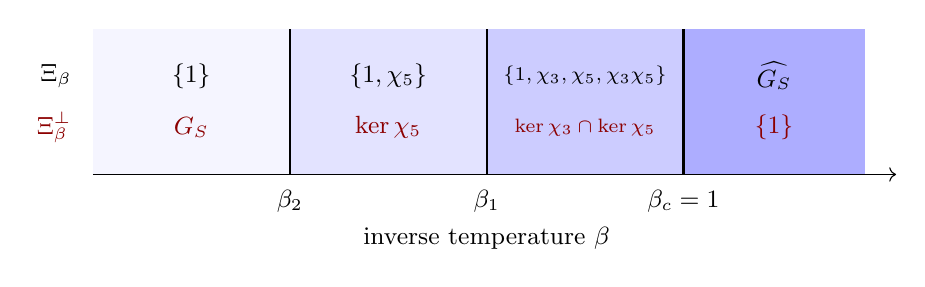
\begin{tikzpicture}[x=1cm, y=1cm]
  \def\ya{0}\def\yb{1.85}\def\xa{1.9}
  \fill[blue!4]  (\xa,\ya)      rectangle (\xa+2.5,\yb);
  \fill[blue!11] (\xa+2.5,\ya)  rectangle (\xa+5.0,\yb);
  \fill[blue!20] (\xa+5.0,\ya)  rectangle (\xa+7.5,\yb);
  \fill[blue!32] (\xa+7.5,\ya)  rectangle (\xa+9.8,\yb);
  \foreach \d in {2.5,5.0,7.5} \draw[thick] (\xa+\d,\ya) -- (\xa+\d,\yb);
  \draw[->] (\xa,\ya) -- (\xa+10.2,\ya);
  \foreach \d/\lab in {2.5/{$\beta_2$}, 5.0/{$\beta_1$}, 7.5/{$\beta_c=1$}}
     \node[below=0.8mm, font=\small] at (\xa+\d,\ya) {\lab};
  \node[below=5.5mm, font=\small] at (\xa+5.0,\ya) {inverse temperature $\beta$};
  \node[anchor=east, font=\small] at (\xa-0.15,1.25) {$\Xi_\beta$};
  \node[anchor=east, font=\small, red!55!black] at (\xa-0.15,0.6) {$\Xi_\beta^{\perp}$};
  \node[font=\small] at (\xa+1.25,1.25) {$\{1\}$};
  \node[font=\small] at (\xa+3.75,1.25) {$\{1,\chi_5\}$};
  \node[font=\scriptsize] at (\xa+6.25,1.25) {$\{1,\chi_3,\chi_5,\chi_3\chi_5\}$};
  \node[font=\small] at (\xa+8.65,1.25) {$\widehat{G_S}$};
  \node[font=\small, red!55!black] at (\xa+1.25,0.6) {$G_S$};
  \node[font=\small, red!55!black] at (\xa+3.75,0.6) {$\ker\chi_5$};
  \node[font=\scriptsize, red!55!black] at (\xa+6.25,0.6) {$\ker\chi_3\cap\ker\chi_5$};
  \node[font=\small, red!55!black] at (\xa+8.65,0.6) {$\{1\}$};
\end{tikzpicture}
\caption{The phase diagram of Proposition~\ref{prop:cascade}. Upper row: the obstruction
group $\Xi_\beta$, increasing with $\beta$ by Lemma~\ref{lem:subgroup}. Lower row: the
residual symmetry group $\Xi_\beta^\perp$, decreasing along the chain. The classical
systems have the single jump $\{1\}\to\widehat{G_S}$ at $\beta=1$.}
\label{fig:cascade}
\end{figure}

\subsection{The unit group and Leopoldt's conjecture}\label{sec:units}

The units enter through the left-hand term of \eqref{eq:exact}, and their effect
is opposite to that of the class group.

\begin{proposition}\label{prop:units}
Enlarging $\overline{\cO^\times_{K,+}}$ shrinks $G_S$, hence $\widehat{G_S}$;
all else equal, this makes the condition $\Xi_\beta(K,S)=\{1\}$ easier to
satisfy. Moreover, let $p$ be a rational prime, suppose $S$ contains every
prime of $K$ above $p$, and let $r$ be the $\Z$-rank of $\cO^\times_{K,+}$.
Then the closure of $\cO^\times_{K,+}$ in $\prod_{\pp\mid p}\cO_\pp^\times$ is a
$\Z_p$-module of rank at most $r$.
\end{proposition}

\begin{proof}
The first statement is immediate from \eqref{eq:exact} and duality: characters
of $G_S$ are characters of $\Idl_S$ trivial on $\overline{K^\times_{S,+}}$, a
stronger condition when the closure is larger. For the second, the closure of a
finitely generated abelian group of rank $r$ inside a $p$-adic Lie group is a
$\Z_p$-module generated by $r$ elements, hence of $\Z_p$-rank at most $r$.
\end{proof}

\begin{remark}\label{rem:leopoldt}
Equality of the rank with $r$ in Proposition~\ref{prop:units} is precisely the
non-vanishing of the $p$-adic regulator, i.e.\ Leopoldt's conjecture for $K$ at
$p$, which is known for $K$ abelian over $\Q$ (Ax--Brumer) and open in general.
We state only the unconditional inequality, and we emphasize that
Theorem~\ref{thm:cheb} is unaffected: the criterion is phrased through
splitting behaviour in finite abelian extensions and does not refer to how the
local units assemble. Leopoldt's conjecture governs the description of $G_S$ as
a topological group, not the classification of its KMS states.
\end{remark}

\subsection{Summary of the comparison}

\[
\begin{array}{lll}
& \Q & \text{general }K\\\hline
\text{parameter group} & \hZ_S^\times & G_S,\ \ 1\to U_S/\overline{\cO^\times_{K,+}}\to G_S\to\Cl^+_S\to1\\
\text{coordinates} & \theta_\ell\ \text{elementary} & \text{ideles; no canonical generator}\\
\text{obstruction test} & \text{Dirichlet character} & \chi(\Frob_\pp),\ \text{ray class character}\\
\text{uniqueness for }S=P_K & \text{Dirichlet} & \text{Chebotarev, i.e.\ }L(1,\chi)\neq0\\
\text{unramified obstructions} & \text{none}\ (h_\Q=1) & \text{subfields of }H^+\text{ when }h^+_K>1\\
\text{units} & \text{trivial} & \text{shrink }G_S,\ \text{aid uniqueness}
\end{array}
\]
\section{Sparse sets: the closed low-temperature phase and Sophie Germain primes}\label{sec:sparse}

We return to $K=\Q$ and apply the theory to sets of primes that are sparse in
the sense of sieve theory. The results of this section concern the location and
nature of the transition rather than the residual symmetry, and they show that
the phase diagram of a localized system can differ from that of \cite{BC} even
when no obstruction group is present.

\begin{definition}\label{def:betac}
The \emph{critical exponent} of a set $S$ of primes is
\[
\beta_c(S)=\inf\Bigl\{\beta>0:\ \sum_{\ell\in S}\ell^{-\beta}<\infty\Bigr\}\in[0,1],
\]
with $\beta_c(S)=0$ if $S$ is finite. We call $S$ \emph{Brun-summable} if
$\sum_{\ell\in S}\ell^{-1}<\infty$.
\end{definition}

\begin{theorem}[Location and nature of the transition]\label{thm:crit}
Let $S$ be a set of primes and $\beta_c=\beta_c(S)$.
\begin{enumerate}
\item For $\beta>\beta_c$ the simplex is $\Prob(G_S)$, with extreme points of
type $\mathrm I_\infty$ permuted freely and transitively by $G_S$
(Theorem~\ref{thm:main}(2)).
\item For $0<\beta<\beta_c$ there are no Gibbs states, and the simplex is
$\Prob(G_S/\Xi_\beta^\perp)$, a point exactly when the criterion of
Theorem~\ref{thm:cheb} holds.
\item $\cA_{\Q,S}$ has a transition, i.e.\ both regimes are nonempty, if and
only if $\beta_c>0$.
\item If $\beta_c>0$ and $\sum_{\ell\in S}\ell^{-\beta_c}<\infty$, then the
type $\mathrm I_\infty$ phase is the \emph{closed} half-line $[\beta_c,\infty)$
and
\[
\lim_{\beta\downarrow\beta_c}\zeta_S(\beta)=\zeta_S(\beta_c)<\infty ,
\]
so the partition function does not diverge at the transition. This hypothesis
holds whenever $S$ is Brun-summable with $\beta_c=1$, since then
$\sum_\ell\ell^{-\beta_c}=\sum_\ell\ell^{-1}<\infty$.
\end{enumerate}
\end{theorem}

\begin{proof}
(1)--(3) are Theorem~\ref{thm:main} and Definition~\ref{def:betac}. For (4), if
$\sum_\ell\ell^{-\beta_c}<\infty$ then $\zeta_S(\beta_c)<\infty$ and
Theorem~\ref{thm:main}(2) applies at $\beta=\beta_c$, so the endpoint lies in
the type $\mathrm I_\infty$ phase. As $\beta\downarrow\beta_c$ one has
$\ell^{-\beta}\uparrow\ell^{-\beta_c}$ for each $\ell$, so by monotone
convergence $\sum_\ell\ell^{-\beta}\to\sum_\ell\ell^{-\beta_c}<\infty$ and the
Euler products converge to $\zeta_S(\beta_c)$. The last sentence is the
definition of Brun-summability together with $\beta_c=1$.
\end{proof}

\begin{remark}\label{rem:sharp}
Item (4) is sharp and marks a genuine difference from the classical system. For
$S$ the set of all primes, $\beta_c=1$ but $S$ is not Brun-summable:
$\sum_\ell\ell^{-1}=\infty$ by Mertens, $\zeta(\beta_c)=\infty$, and
$\zeta(\beta)\to\infty$ as $\beta\downarrow1$ through the pole. Thus:
\[
\begin{array}{lccc}
& \beta_c & \zeta_S(\beta_c) & \text{phase of }\beta_c\\\hline
\text{all primes (Bost--Connes)} & 1 & \infty & \text{high-temperature}\\
\text{Brun-summable with }\beta_c=1 & 1 & <\infty & \text{type }\mathrm I_\infty
\end{array}
\]
The two systems have the same critical temperature and opposite behaviour at
it; the critical point belongs to the symmetric phase in one case and to the
symmetry-broken phase in the other. The distinction is invisible in the
exponent: it is the difference between Mertens' theorem and Brun's theorem.
\end{remark}

\begin{remark}
For $0<\beta_c<1$ the value $\zeta_S(\beta_c)$ is not determined by $\beta_c$
alone; both convergence and divergence occur among sets with the same
convergence exponent, as one sees by comparing $\ell_k\approx\exp(k^{1/\beta_c})$
with $\ell_k\approx\exp(k^{1/\beta_c}/\log k)$. The Brun-summable case with
$\beta_c=1$ is the one relevant below.
\end{remark}

\begin{figure}[htbp]
\centering
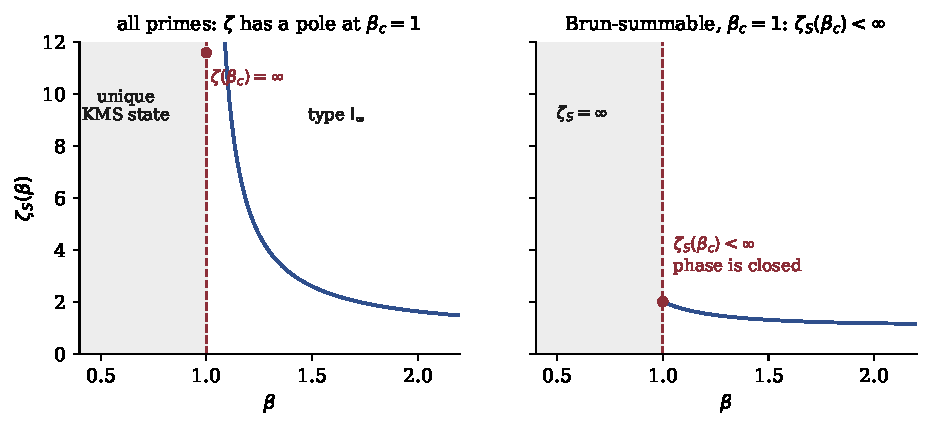
\includegraphics[width=\textwidth]{fig1_closed_vs_open_phase.pdf}
\caption{Remark~\ref{rem:sharp}: the same critical temperature, opposite
behaviour at it. Left, the classical system, where $\zeta$ has a pole at
$\beta_c=1$ and the critical point lies in the high-temperature phase. Right, a
Brun-summable set with $\beta_c=1$, where $\zeta_S(\beta_c)<\infty$ and the type
$\mathrm I_\infty$ phase is closed.}
\label{fig:closed}
\end{figure}

\subsection{Sophie Germain primes}

Let $\SG=\{p\ \text{prime}:2p+1\ \text{prime}\}$, $\pi_\SG(x)=|\SG\cap[1,x]|$,
and $S_\infty=\{2\}\cup\SG$; by Proposition~\ref{prop:indlim},
$\cA_{\Q,S_\infty}=\varinjlim_k\cA_{\Q,T_k}$ with $T_k=\{2,p_1,\dots,p_k\}$,
and $\cA_{\Q,S_\infty}\subseteq\cA_{BC}$.

\begin{theorem}\label{thm:sg}
Let $\beta_c=\beta_c(S_\infty)$.
\begin{enumerate}
\item \emph{(Unconditional.)} $\pi_\SG(x)\ll x/\log^2x$ \cite{HR}; hence
$S_\infty$ is Brun-summable, $\zeta_{S_\infty}(\beta)<\infty$ for all
$\beta\ge1$, and $\beta_c\le1$.
\item If $\pi_\SG(x)\gg x/\log^Ax$ for some $A>0$---in particular under the
Hardy--Littlewood conjecture $\pi_\SG(x)\sim2C_2\,x/\log^2x$ \cite{HL}---then
$\beta_c=1$.
\item Under the hypothesis of (2), $\zeta_{S_\infty}$ is finite on $[1,\infty)$
and identically $+\infty$ on $(0,1)$, and the type $\mathrm I_\infty$ phase of
$\cA_{\Q,S_\infty}$ is exactly $[1,\infty)$: a closed low-temperature phase
whose critical point is $\beta_c=1$.
\item $\cA_{\Q,S_\infty}$ has a phase transition if and only if $\SG$ has
positive convergence exponent; in particular a phase transition implies that
$\SG$ is infinite.
\item For $\beta$ in the range where $\zeta_{S_\infty}(\beta)=\infty$, the
$\mathrm{KMS}_\beta$ state is unique if and only if, for every modulus $M$
supported on $S_\infty$ and every proper subgroup $H<(\Z/M\Z)^\times$,
\[
\sum_{\substack{p\in\SG\\ p\bmod M\notin H}}p^{-\beta}=\infty ;
\]
this holds under the Hardy--Littlewood conjecture with congruence conditions.
\end{enumerate}
\end{theorem}

\begin{proof}
(1) Abel summation: with $\pi_\SG(t)\le Ct/\log^2t$ for $t\ge t_0$,
\[
\sum_{p\in\SG,\ p\le x}\frac1p=\frac{\pi_\SG(x)}{x}+\int_{t_0}^x\frac{\pi_\SG(t)}{t^2}\,dt+O(1)
\le O(1)+C\int_{t_0}^x\frac{dt}{t\log^2t}=O(1).
\]
Hence $\sum_{p\in\SG}p^{-1}<\infty$, $\beta_c\le1$, and
$\zeta_{S_\infty}(\beta)<\infty$ for $\beta\ge1$ since $\ell^{-\beta}\le\ell^{-1}$.

(2) For $0<\beta<1$, Abel summation with the lower bound gives
\[
\sum_{p\in\SG,\ p\le x}p^{-\beta}\ \ge\ \beta\int_{t_0}^x\frac{\pi_\SG(t)}{t^{\beta+1}}\,dt
\ \gg\ \int_{t_0}^x\frac{dt}{t^{\beta}\log^At}\ \gg\ \frac{x^{1-\beta}}{\log^Ax}\longrightarrow\infty,
\]
so $\beta_c\ge1$; with (1), $\beta_c=1$.

(3) Combine (1), (2) and Theorem~\ref{thm:crit}(4).

(4) Theorem~\ref{thm:crit}(3).

(5) The first assertion is Theorem~\ref{thm:cheb} specialized to $K=\Q$, where
the abelian extensions unramified outside $S\cup\infty$ are the subfields of
cyclotomic fields $\Q(\zeta_M)$ with $M$ supported on $S$, and $\Frob_p$ is the
class of $p$ modulo $M$. For the conditional statement, assume that for each
admissible residue $a$ one has
$|\{p\le x:p\in\SG,\ p\equiv a\ (M)\}|\gg_Mx/\log^2x$, where
\[
A_M=\{a\in(\Z/M\Z)^\times:\ 2a+1\in(\Z/M\Z)^\times\}
\]
is the set of admissible classes. By Lemma~\ref{lem:admissible} below,
$\langle A_M\rangle=(\Z/M\Z)^\times$, so for any proper subgroup $H$ there is
$a\in A_M\setminus H$; the primes of $\SG$ in that class then give a divergent
sum by the computation in (2), and they all lie outside $H$.
\end{proof}

\begin{lemma}\label{lem:admissible}
$\langle A_M\rangle=(\Z/M\Z)^\times$ for every $M\ge1$.
\end{lemma}

\begin{proof}
Let $\chi$ be a character of $(\Z/M\Z)^\times$ trivial on $A_M$; we show
$\chi=1$. By the Chinese remainder theorem, $\chi=\prod_\ell\chi_\ell$ and
$A_M=\prod_\ell A_{\ell^{k_\ell}}$, where $A_{2^k}=(\Z/2^k)^\times$ and, for
$\ell$ odd, $A_{\ell^k}=\{a\in(\Z/\ell^k)^\times:a\not\equiv-2^{-1}\bmod\ell\}$.
As $A_M$ is a product, each $\chi_\ell$ is constant on $A_{\ell^{k_\ell}}$, say
with value $c_\ell$, and $\prod_\ell c_\ell=1$.

For $\ell=2$: $A_{2^k}$ is the whole group, so $\chi_2=1$ and $c_2=1$. For
$\ell\ge5$: $|A_{\ell^k}|=\varphi(\ell^k)(1-\frac{1}{\ell-1})>\frac12\varphi(\ell^k)$,
so $A_{\ell^k}A_{\ell^k}^{-1}=(\Z/\ell^k)^\times$, and $\chi_\ell$, being
constant on $A_{\ell^k}$, is trivial, so $c_\ell=1$. For $\ell=3$:
$A_{3^k}=\{a:a\not\equiv1\bmod3\}$ is the nontrivial coset of the index-two
subgroup $K=\{a\equiv1\bmod3\}$, so $A_{3^k}A_{3^k}^{-1}=K$ and $\chi_3$ is
trivial on $K$; hence $\chi_3$ is trivial or the quadratic character with
kernel $K$, and $c_3=\pm1$ accordingly. Since all other $c_\ell=1$ and
$\prod c_\ell=1$, we get $c_3=1$, so $\chi_3$ is trivial on $A_{3^k}\cup K$,
which is everything. Therefore $\chi=1$.
\end{proof}

\begin{remark}\label{rem:noroute}
Theorem~\ref{thm:sg}(4) is an equivalence, not an implication in a useful
direction. Establishing the transition requires exactly the arithmetic input
that is unavailable, a lower bound on the density of $\SG$; and the transition,
once granted, yields nothing about $\SG$ beyond the density statement assumed.
The construction is a dictionary entry, not a method. The same applies verbatim
to the twin primes, to the primes $p$ with $p+2k$ prime for fixed $k$, and to
any set for which a Brun-type upper bound is known and a matching lower bound
conjectured: all such systems have the same phase diagram, and none of them
distinguishes its defining condition from any other of the same density. What
Theorem~\ref{thm:sg} does record is that the two open points---the location of
$\beta_c$ and the uniqueness below it---are governed by the same input, the
second in a form refined by congruence conditions.
\end{remark}

\begin{figure}[htbp]
\centering
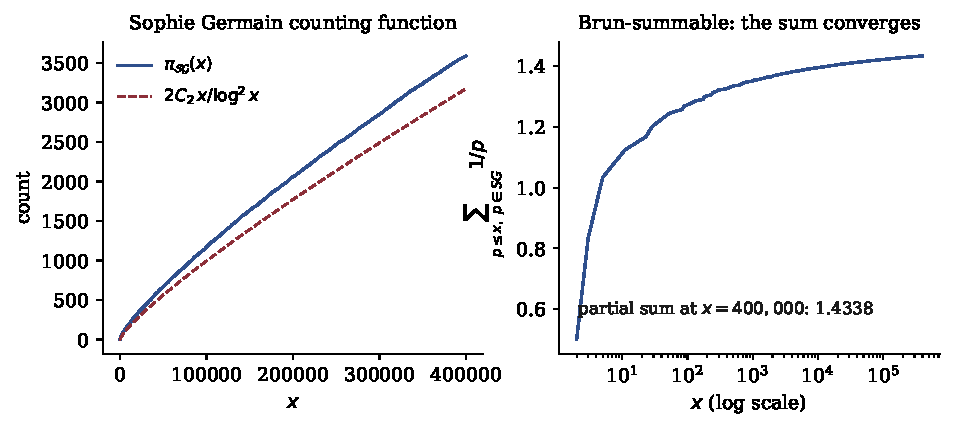
\includegraphics[width=\textwidth]{fig4_sophie_germain.pdf}
\caption{Data for Theorem~\ref{thm:sg}(1). Left, $\pi_\SG(x)$ against
$2C_2x/\log^2x$. Right, the partial sums of $\sum_{p\in\SG}1/p$, whose
convergence is the Brun-summability used throughout \S\ref{sec:sparse}.}
\label{fig:sg}
\end{figure}

\subsection{Restriction of the classical phases}

Finally we record how the phases of the full system restrict, which explains in
what sense the localized systems are cross-sections of the classical one.

\begin{proposition}\label{prop:restr}
Let $S$ be a set of primes with complement $S^c$, let $\beta>1$ and
$\chi\in\hZ^\times$, and let $\varphi^{BC}_{\beta,\chi}$ be the corresponding
extremal $\mathrm{KMS}_\beta$ state of $\cA_{BC}$. Then, under the embedding of
Proposition~\ref{prop:indlim},
\[
\varphi^{BC}_{\beta,\chi}\big|_{\cA_{\Q,S}}
=\frac1{\zeta_{S^c}(\beta)}\sum_{m\in\N_{S^c}}m^{-\beta}\,\varphi^{S}_{\beta,\,\mathrm{pr}_S(m)\chi_S},
\qquad\chi_S=\mathrm{pr}_S(\chi).
\]
The map $\chi_S\mapsto\varphi^{BC}_{\beta,\chi}|_{\cA_{\Q,S}}$ is injective and
$\hZ_S^\times$-equivariant, but if $S^c$ is infinite its image consists
entirely of non-extremal states, whose measures have infinitely many atoms. For
$0<\beta\le1$ the unique $\mathrm{KMS}_\beta$ state of $\cA_{BC}$ restricts to
the symmetric state of $\cA_{\Q,S}$.
\end{proposition}

\begin{proof}
Decompose $\ell^2(\N^\times)=\bigoplus_{m\in\N_{S^c}}\ell^2(m\N_S)$. Each
summand is invariant under $\pi_\chi(\cA_{\Q,S})$, and $\epsilon_{mn}\mapsto\epsilon_n$
intertwines $\pi_\chi|_{\cA_{\Q,S}}$ on $\ell^2(m\N_S)$ with
$\pi_{\mathrm{pr}_S(m)\chi_S}$, while $e^{-\beta H}$ restricts to
$m^{-\beta}e^{-\beta H_S}$. Summing and using $\zeta=\zeta_S\zeta_{S^c}$ gives
the formula. The atoms $\mathrm{pr}_S(m)\chi_S$ are pairwise distinct, since
$\mathrm{pr}_S(m)=\mathrm{pr}_S(m')$ forces $m\equiv m'$ modulo $\ell^k$ for all
$\ell\in S$ and all $k$, hence $m=m'$; the atom of largest mass is the one with
$m=1$, so $\chi_S$ is recoverable, and equivariance follows from
$\pi_\chi\circ\theta_v=\pi_{v^{-1}\chi}$. Extremal states correspond to point
masses by Theorem~\ref{thm:main}(2), whereas these measures have infinitely
many atoms when $\N_{S^c}$ is infinite. The last claim follows from
$\hZ^\times$-invariance of the unique state.
\end{proof}

\begin{remark}
So the parameter space of the low-temperature phase projects equivariantly,
$\hZ^\times\to\hZ_S^\times$, and this is a genuine reduction of the Galois
symmetry; what does not descend is extremality, because the degrees of freedom
at the primes outside $S$ have been traced out rather than fixed. In
particular the transition of $\cA_{\Q,S}$ at $\beta_c(S)$ is not the
restriction of the transition of $\cA_{BC}$ at $\beta=1$: for Brun-summable $S$
with $\beta_c(S)=1$ the two occur at the same temperature but on opposite
sides, by Remark~\ref{rem:sharp}.
\end{remark}

\section{Assessment and open problems}\label{sec:assessment}

We separate what is established from what is not.

\emph{Established unconditionally.} Theorem~\ref{thm:main} classifies the
$\mathrm{KMS}_\beta$ states of $\cA_{K,S}$ for every number field $K$, every
set $S$ of finite primes and every $\beta>0$; Theorem~\ref{thm:cheb} converts
it into the splitting criterion; Corollary~\ref{cor:full} recovers the
classical theorems of \cite{BC,LLN} from Chebotarev; Example~\ref{ex:first},
Theorem~\ref{thm:dens} and Example~\ref{ex:sqrt5} exhibit failures of
uniqueness with divergent partition function, the last two with dense
$\sigma(I_S)$; Proposition~\ref{prop:Psi} supplies the invariant;
Theorem~\ref{thm:crit} locates the transition and shows the low-temperature
phase can be closed; Theorem~\ref{thm:sg}(1) is unconditional.

\emph{Conditional or incomplete.} Theorem~\ref{thm:sg}(2),(3),(5) depend on a
lower bound for $\pi_\SG$ of Hardy--Littlewood strength, in (5) refined by
congruence conditions; Remark~\ref{rem:leopoldt} records that the description of $G_S$ as a
topological group, though not the criterion, is entangled with Leopoldt's
conjecture.

\emph{Relation to the literature.} Sections \ref{sec:system} and \ref{sec:crit} are, for
$S=P_K$, a reformulation of results in \cite{BC,LR,LLN,Nesh13,Nesh02}; the reduction to
measures (Proposition~\ref{prop:kmsmeasures}) uses \cite{Laca} and \cite{Nesh13} directly.
It is worth stating precisely where the present work goes beyond \cite{Nesh13}. That paper
classifies KMS states on $C^*$-algebras of \emph{non-principal} groupoids, and its content
lies in the field of states on the isotropy group algebras. Proposition~\ref{prop:kmsmeasures}
shows that our groupoid is principal on a conull set---the $I_S$-action is free because the
valuation vector is translated freely---so the isotropy data is empty and \cite{Nesh13}
contributes only the reduction to quasi-invariant measures. Everything after that point is
independent of it: the forced product structure of the valuation marginal
(Lemma~\ref{lem:coords}(3)), the cohomological equation \eqref{eq:coc}, and the extraction
of the arithmetic obstruction group $\Xi_\beta$ from a Kakutani product criterion
(Propositions~\ref{prop:nec} and \ref{prop:suff}) are what produce Theorem~\ref{thm:main},
and we have found no counterpart to them in \cite{Nesh13}. A literature check remains
advisable, but the boundary is clear enough that we do not expect a conflict.

\emph{The type of the intermediate phases.} We record what the ratio-set argument does and
does not give.

\begin{proposition}\label{prop:type}
Let $\beta>0$ with $\zeta_{K,S}(\beta)=\infty$, let $\varphi$ be an extremal
$\mathrm{KMS}_\beta$ state of $\cA_{K,S}$, and let $M=\pi_\varphi(\cA_{K,S})''$. Put
\[
\Gamma_\beta=\bigl\langle \Ns\pp^{-\beta}:\pp\in S\bigr\rangle\ \le\ \R_{>0}.
\]
Then $M$ is a factor of type $\mathrm{III}$, and its Connes invariant satisfies
\[
S(M)\ \subseteq\ \overline{\Gamma_\beta}\cup\{0\}.
\]
Consequently, if the numbers $\log\Ns\pp$, $\pp\in S$, are pairwise commensurable and
generate $\log\lambda_0\cdot\Z$, then $S(M)\subseteq\{0\}\cup\lambda_0^{-\beta\Z}$, so $M$ is of type
$\mathrm{III}_{\lambda_0^{-n\beta}}$ for some integer $n\ge1$ or of type $\mathrm{III}_0$.
\end{proposition}

\begin{proof}
Extreme points of a KMS simplex give factor states \cite[\S5.3]{BR}. By
Proposition~\ref{prop:kmsmeasures} the groupoid is principal on a conull set, so $M$ is
the Krieger factor of the orbit equivalence relation of $I_S$ acting on $(Y_S,\nu)$, and by
Krieger's theorem \cite{Krieger} $S(M)$ is the ratio set of that relation. The Radon--Nikodym cocycle is
$\aaa\bb^{-1}\mapsto(\Ns\aaa/\Ns\bb)^{-\beta}$, whose values lie in $\Gamma_\beta$; the
ratio set is contained in the closure of the essential range of the cocycle, hence in
$\overline{\Gamma_\beta}\cup\{0\}$.

$M$ is not semifinite. By \cite{Krieger} this means that the relation carries no
$\sigma$-finite invariant measure equivalent to $\nu$, i.e.\ that there is no measurable
$f:Y_S\to(0,\infty)$ with $f(\aaa\cdot y)=\Ns\aaa^{\beta}f(y)$ for $\nu$-a.e.\ $y$ and all
$\aaa\in J_S$. Suppose $f$ exists and put $X=\log f$. In the coordinates of
Lemma~\ref{lem:coords}, the function
$\Phi(v,t):=\int_{G_S}e^{itX(v,g)}\,d\rho_v(g)$ satisfies, by \eqref{eq:coc} and
Lemma~\ref{lem:coords}(2), $\Phi(v+a,t)=\Ns\aaa^{i\beta t}\,\Phi(v,t)$ for $\pi_\beta$-a.e.\ $v$:
this is \eqref{eq:fchi} with $\overline{\chi(\sigma_\aaa)}$ replaced by the unimodular
constants $c_\aaa=\Ns\aaa^{i\beta t}$, and the proofs of Lemma~\ref{lem:01} and
Proposition~\ref{prop:nec} use nothing else. Fix $t$, write $c_\pp=\Ns\pp^{i\beta t}$ and
$m_\pp(t)=(1-t_\pp)/(1-c_\pp t_\pp)$. As in the proof of Proposition~\ref{prop:nec}, for
every finite $F\subset S$ we have $\Phi=P_F\,G_F$ with $P_F=\prod_{\pp\in F}c_\pp^{v_\pp}$ and
$G_F$ measurable with respect to $\sigma(v_\pp:\pp\notin F)$, hence independent of $P_F$ and
bounded by $1$. Therefore
\[
\psi(t):=\int_{Y_S}e^{itX}\,d\nu=\mathbb{E}_{\pi_\beta}\bigl[\Phi(\cdot,t)\bigr]=\mathbb{E}[P_F]\,\mathbb{E}[G_F],
\qquad |\psi(t)|\le\prod_{\pp\in F}|m_\pp(t)|,
\]
and letting $F\uparrow S$ and using Lemma~\ref{lem:mp} in the form
$1-|m_\pp|\ge\frac12(1-|m_\pp|^2)\ge\frac18t_\pp|1-c_\pp|^2$,
\[
|\psi(t)|\ \le\ \prod_{\pp\in S}|m_\pp(t)|\ \le\ \exp\Bigl(-\tfrac18\,g(t)\Bigr),\qquad
g(t):=\sum_{\pp\in S}\Ns\pp^{-\beta}\,\bigl|1-\Ns\pp^{i\beta t}\bigr|^2 .
\]
Now $\psi$ is the characteristic function of the law of $X$ under $\nu$, so it is continuous
with $\psi(0)=1$; choose $\delta>0$ with $|\psi|\ge\frac12$ on $[0,\delta]$. Then
$g\le8\log2$ on $[0,\delta]$. But $|1-e^{i\omega t}|^2=4\sin^2(\omega t/2)$ and
$\int_0^\delta4\sin^2(\omega t/2)\,dt=2\delta-\frac2\omega\sin(\omega\delta)\ge\delta$ as
soon as $\omega\delta\ge2$, so by Tonelli
\[
\int_0^\delta g(t)\,dt\ \ge\ \delta\sum_{\pp\in S:\ \beta\delta\log\Ns\pp\ge2}\Ns\pp^{-\beta}
\ =\ \infty,
\]
the sum omitting only finitely many primes of $S$ and $\zeta_{K,S}(\beta)=\infty$. This
contradicts $g\le8\log2$ on $[0,\delta]$, so no such $f$ exists and $M$ is of type
$\mathrm{III}$.

For the last statement, a closed subgroup of $\lambda_0^{-\beta\Z}$ is $\lambda_0^{-n\beta\Z}$
for some $n\ge0$; $n=0$ would give $S(M)\subseteq\{0,1\}$, i.e.\ type $\mathrm{III}_0$, and
$n\ge1$ gives type $\mathrm{III}_{\lambda_0^{-n\beta}}$.
\end{proof}

\begin{remark}\label{rem:typewarning}
Proposition~\ref{prop:type} bounds $S(M)$ from \emph{above}. It is tempting to argue that
when two norms have irrational log-ratio, $\Gamma_\beta$ is dense in $\R_{>0}$ and therefore
$S(M)=[0,\infty)$, i.e.\ $M$ is $\mathrm{III}_1$; but this inference is invalid, since
density of the group of \emph{possible} ratios gives no lower bound on the ratio set, and
$\mathrm{III}_0$---where $S(M)=\{0,1\}$---is not excluded. Establishing $\mathrm{III}_1$
requires the ergodicity of the Maharam extension of the action, equivalently that the
essential range of the cocycle is all of $\overline{\Gamma_\beta}$.

The natural candidate for the missing ingredient is an \emph{extended} obstruction group
$\Xi_\beta^{\mathrm{ext}}\le\widehat{G_S}\times\R$, obtained from \eqref{eq:Xi} by twisting
the characters with $\Ns\pp^{\,i\beta s}$ and having $\Xi_\beta$ as its $s=0$ slice; the
essential range of the cocycle should be readable from its projection to $\R$. We do not
pursue this here, and nothing in this paper depends on it. Note that the commensurable case
of Proposition~\ref{prop:type} is vacuous once $S$ is infinite, since $\log p$ for distinct
rational primes are $\Q$-linearly independent and only finitely many primes of $K$ lie
above each $p$; any failure of type $\mathrm{III}_1$ arises from \emph{approximate}
commensurability along a set of divergent $\beta$-weight.
\end{remark}

\emph{Open problems.}
\begin{enumerate}
\item Determine the type of the extremal states. Proposition~\ref{prop:type} bounds $S(M)$
from above and Remark~\ref{rem:typewarning} explains what a lower bound requires; for the
sparse sets of \S\ref{sec:sparse} it is not decided here which of the alternatives
$\mathrm{III}_1$, $\mathrm{III}_\lambda$, $\mathrm{III}_0$ occurs.
\item Characterize the possible chains $\{\Xi_\beta\}_{\beta>0}$. By
Lemma~\ref{lem:subgroup} they are increasing; Proposition~\ref{prop:cascade} realizes
finite chains. The transition set is always countable, $\widehat{G_S}$ being countable;
which monotone families of subgroups of $\widehat{G_S}$ occur, and whether infinitely many
transitions can be forced into a bounded interval, are open.
\item Extend the criterion to the function field case, where Chebotarev is
available with error terms from the Riemann hypothesis for curves, and where
sparse sets of closed points can be constructed with more freedom than sparse
sets of primes. One structural difference is worth recording: the log-norms
$\log\Ns P=\deg P\cdot\log q$ are pairwise commensurable, so the commensurable case of
Proposition~\ref{prop:type}---vacuous over a number field by
Remark~\ref{rem:typewarning}---is there the only case.
\item In Example~\ref{ex:sqrt5} the obstruction is unramified. Is there a
canonical description of the sub-simplex of $\mathrm{KMS}_\beta$ states cut out
by the unramified part of $\widehat{G_S}$, in terms of the Hilbert class field,
valid for all $S$ simultaneously?
\end{enumerate}

\begin{thebibliography}{99}
\bibitem{BC} J.-B. Bost, A. Connes, \emph{Hecke algebras, type III factors and phase transitions with spontaneous symmetry breaking in number theory}, Selecta Math. (N.S.) 1 (1995), 411--457.
\bibitem{BR} O. Bratteli, D. W. Robinson, \emph{Operator Algebras and Quantum Statistical Mechanics 2}, 2nd ed., Springer, 1997.
\bibitem{Fur} H. Furstenberg, \emph{Strict ergodicity and transformations of the torus}, Amer. J. Math. 83 (1961), 573--601.
\bibitem{Hecke} E. Hecke, \emph{Eine neue Art von Zetafunktionen und ihre Beziehungen zur Verteilung der Primzahlen}, Math. Z. 1 (1918), 357--376; 6 (1920), 11--51.
\bibitem{Landau} E. Landau, \emph{\"Uber Ideale und Primideale in Idealklassen}, Math. Z. 2 (1918), 52--154.
\bibitem{Krieger} W. Krieger, \emph{On ergodic flows and the isomorphism of factors}, Math. Ann. 223 (1976), 19--70.
\bibitem{HP} E. Ha, F. Paugam, \emph{Bost--Connes--Marcolli systems for Shimura varieties}, IMRP 2005, no.~5, 237--286.
\bibitem{HL} G. H. Hardy, J. E. Littlewood, \emph{Some problems of `Partitio numerorum'; III}, Acta Math. 44 (1923), 1--70.
\bibitem{HR} H. Halberstam, H.-E. Richert, \emph{Sieve Methods}, Academic Press, 1974.
\bibitem{Laca} M. Laca, \emph{From endomorphisms to automorphisms and back: dilations and full corners}, J. London Math. Soc. (2) 61 (2000), 893--904.
\bibitem{LLN} M. Laca, N. S. Larsen, S. Neshveyev, \emph{On Bost--Connes type systems for number fields}, J. Number Theory 129 (2009), 325--338.
\bibitem{LR} M. Laca, I. Raeburn, \emph{A semigroup crossed product arising in number theory}, J. London Math. Soc. (2) 59 (1999), 330--344.
\bibitem{Nesh02} S. Neshveyev, \emph{Ergodicity of the action of the positive rationals on the group of finite adeles and the Bost--Connes phase transition theorem}, Proc. Amer. Math. Soc. 130 (2002), 2999--3003.
\bibitem{Nesh13} S. Neshveyev, \emph{KMS states on the $C^*$-algebras of non-principal groupoids}, J. Operator Theory 70 (2013), 513--530.
\bibitem{Neu} J. Neukirch, \emph{Algebraic Number Theory}, Grundlehren 322, Springer, 1999.
\end{thebibliography}

\end{document}
